\documentclass[a4paper]{article}
\usepackage[normalem]{ulem}
\usepackage{graphicx}
\usepackage[font=small,labelfont=bf]{caption}

% impostazioni generali
%Tutti gli usepackage vanno qui
\usepackage[table]{xcolor}
\usepackage{geometry}
\usepackage[italian]{babel}
\usepackage[utf8]{inputenc}
\usepackage{tabularx}
\usepackage{longtable}
\usepackage{hyperref}
\usepackage{enumitem}
\usepackage{array} 
\usepackage{booktabs}
\newcolumntype{M}[1]{>{\centering\arraybackslash}m{#1}}
\usepackage[toc]{appendix}
\usepackage{caption}

\hypersetup{
	colorlinks=true,
	linkcolor=blue,
	filecolor=magenta,
	urlcolor=blue,
}
% Numerazione figure
\let\counterwithout\relax
\let\counterwithin\relax
\usepackage{chngcntr}

% distanziare elenco delle figure e delle tabelle
\usepackage{tocbasic}
\DeclareTOCStyleEntry[numwidth=3.5em]{tocline}{figure}% for figure entries
\DeclareTOCStyleEntry[numwidth=3.5em]{tocline}{table}% for table entries


%\counterwithout{table}{section}
%\counterwithout{figure}{section}
\captionsetup[table]{font=small,skip=5pt} 

\usepackage[bottom]{footmisc}
\usepackage{fancyhdr}
\setcounter{secnumdepth}{4}
\usepackage{amsmath, amssymb}
\usepackage{array}
\usepackage{graphicx}

\usepackage{ifthen}

\usepackage{float}
\restylefloat{table}

\usepackage{layouts}
\usepackage{url}
\usepackage{comment}
\usepackage{eurosym}

\usepackage{lastpage}
\usepackage{layouts}
\usepackage{eurosym}

\geometry{a4paper,top=3cm,bottom=4cm,left=2.5cm,right=2.5cm}

%Comandi di impaginazione uguale per tutti i documenti
\pagestyle{fancy}
\lhead{
\includegraphics[scale=0.25]{template/images/logo-inline.png}}


%\rfoot{\thepage}
\cfoot{Pagina \thepage\ di \pageref{LastPage}}
\setlength{\headheight}{35pt}
\setcounter{tocdepth}{5}
\setcounter{secnumdepth}{5}
\renewcommand{\footrulewidth}{0.4pt}

% multirow per tabelle
\usepackage{multirow}

% Permette tabelle su più pagine
%\usepackage{longtable}


%COMANDI TABELLE
\newcommand{\rowcolorhead}{\rowcolor[HTML]{731733}}
\newcommand{\captionline}{\rowcolor[HTML]{FFFFFF}} %comando per le caption delle tabelle
\newcommand{\cellcolorhead}{\cellcolor[HTML]{007c95}}
\newcommand{\hlinetable}{\arrayrulecolor[HTML]{007c95}\hline}

%intestazione
% check for missing commands
\newcommand{\headertitle}[1]{\textbf{\color{white}#1}} %titolo colonna
\definecolor{pari}{HTML}{dcbac2}
\definecolor{dispari}{HTML}{f5f5f5}

% comandi \textit{Glossario}
\newcommand{\glo}{$_{G}$}
\newcommand{\glosp}{$_{G}$ }


%label custom
\makeatletter
\newcommand{\uclabel}[2]{%
	\protected@write \@auxout {}{\string \newlabel {#1}{{#2}{\thepage}{#2}{#1}{}} }%
	\hypertarget{#1}{#2}
}
\makeatother

%riportare pezzi di codice
\definecolor{codegray}{gray}{0.9}
\newcommand{\code}[1]{\colorbox{codegray}{\texttt{#1}}}

% dati relativi alla prima pagina
\makeindex


\begin{document}
\counterwithin{table}{section}

% Prima pagina
\thispagestyle{empty}
\renewcommand{\arraystretch}{1.3}


\begin{titlepage}
	\begin{center}
		
	
\includegraphics[scale = 0.7]{template/images/logo-circle.png}
	\\[1cm]
	\href{mailto:6bitbusters@gmail.com}		      	
	{\large{\textit{6bitbusters@gmail.com} } }\\[1cm]
	
	\Huge \textbf{Analisi dei requisiti} \\[1cm]

	% Informazioni sul documento
	\large \textbf{Informazioni sul documento} \\
	\rule{0.6\textwidth}{0.4pt}
	\\[0.5cm]
	\begin{tabular}{r|l}
		\textbf{Versione} & 0.8.0\\
		\textbf{Stato} & in redazione\\
		\textbf{Uso} & esterno\\                         
		\textbf{Approvazione} & -\\                      
		\textbf{Redazione} & Pincin Matteo\\ & Diviesti Filippo\\ & Soranzo Andrea \\ & Djossa Edgar \\
		\textbf{Verifica} & Bergamin Elia\\ & Soranzo Andrea \\ & Chilese Elena \\  & Djossa Edgar \\                     
		\textbf{Distribuzione} & \parbox[t]{5cm}{ \textit{Six Bit Busters} \\ Prof. Vardanega Tullio 
	 \\ Prof. Cardin Riccardo}
	\end{tabular}	
	\\[1.2cm]

 % Descrizione
	\large \textbf{Descrizione} \\ Documento di rendicontazione dell'\textit{Analisi dei requisiti}
	
	
	\end{center}
\end{titlepage}


% Diario delle modifiche

\section*{Registro delle modifiche}

\newcommand{\changelogTable}[1]{

\renewcommand{\arraystretch}{1.5}
\rowcolors{2}{pari}{dispari}
\begin{longtable}{ %0.87
		>{\centering}M{0.10\textwidth} 
		>{\centering}M{0.11\textwidth}
		>{\centering}M{0.19\textwidth}
		>{\centering}M{0.28\textwidth} 
		>{\centering\arraybackslash}M{0.19\textwidth} 
		 }
	\rowcolorhead
	\headertitle{Versione} &
	\centering \headertitle{Data} &	
	\headertitle{Autore} &
	\headertitle{Descrizione} & 
	\headertitle{Verificatore} 
	\endfirsthead	
	\endhead
	
	#1

\end{longtable}
\vspace{-2em}

}
% Insert changelog values here
\changelogTable{
  2.0.1 & 19-03-2025 & Soranzo Andrea & Rimossi numeri di sezione & - \tabularnewline
  2.0.0 & 02-03-2025 & Soranzo Andrea & Approvazione documento & - \tabularnewline
	1.1.0 & 02-03-2025 & Bergamin Elia & Integrazione vocaboli & Djossa Edgar \tabularnewline
	1.0.0 & 31-01-2025 & Soranzo Andrea & Approvazione documento & - \tabularnewline
	0.7.0 & 30-01-2025 & Chilese Elena & Revisione documento & Bergamin Elia \tabularnewline
	0.6.0 & 28-01-2025 & Bergamin Elia & Integrazione vocaboli & Pincin Matteo \tabularnewline
	0.5.0 & 10-01-2025 & Diviesti Filippo & Integrazione vocaboli & Soranzo Andrea\tabularnewline
    0.4.0 & 16-12-2024 & Djossa Edgar & Integrazione vocaboli & Chilese Elena \tabularnewline   
	0.3.0 & 10-12-2024 & Bergamin Elia & Aggiunta Introduzione, integrazione vocaboli e morfologia & Djossa Edgar \tabularnewline
	0.2.0 & 25-11-2024 & Bergamin Elia & Integrazione vocaboli & Soranzo Andrea \tabularnewline
	0.1.0 & 19-11-2024 & Diviesti Filippo & Inserimento vocaboli per \textit{Norme di progetto} e \textit{Piano di progetto} & Pincin Matteo \\
}

\pagebreak

% Indice
{
    \hypersetup{linkcolor=black}
    \tableofcontents
}
\pagebreak

\section{Introduzione}
\subsection{Scopo del documento}
Questo documento ha lo scopo di descrivere le scelte progettuali fondamentali
per la struttura, il comportamento e l'interoperabilità del sistema software.
In particolare, serve a:
\begin{itemize}
      \item Definire i moduli, le componenti, le loro responsabilit`a e le interazioni;
      \item Fornire un riferimento agli sviluppatori per implementare il software in modo
            coerente;
      \item Garantire la completa copertura dei requisiti individuati nell'\textit{Analisi
                  dei requisiti v2.0.0}.
\end{itemize}
A tale scopo, il documento descrive le tecnologie selezionate, l'architettura implementativa e l'architettura
di deployment. Ciò include la descrizione delle classi, dei design pattern e delle librerie utilizzate, anche
con l'ausilio di diagrammi UML.

\subsection{Scopo del prodotto}
\textit{3Dataviz} è un prodotto ideato dall'azienda \textit{Sanmarco Informatica S.p.A.} per semplificare e rendere più accessibile la visualizzazione dei dati.\\
Esso mira a trasformare i dati in grafici e rappresentazioni visive, sfruttando la capacità del cervello umano di elaborare rapidamente le immagini.
Questo approccio facilita il processo decisionale e migliora la comprensione delle informazioni.\\
L'obiettivo principale è lo sviluppo di un'interfaccia web che trasforma dati provenienti da diverse fonti (come database e REST API) in grafici 3D interattivi e navigabili.
I dati potranno essere consultati anche in formato tabellare, offrendo una visione alternativa ma altrettanto utile.

\subsection{Glossario}
Per chiarire i termini tecnici o ambigui si utilizza un glossario disponibile
nel file \textit{Glossario v2.0.0}.\\ Tutti i termini che richiedono
spiegazioni sono indicati con il pedice “g”. \\ Questa convenzione consente un
rapido collegamento tra il testo e la relativa spiegazione dettagliata nel
glossario, garantendo coerenza e chiarezza.

\subsection{Riferimenti normativi}
\begin{itemize}
      \item \textit{Norme di progetto v2.0.0} \\ \url{https://6bitbusters.github.io/norme_di_progetto.pdf}
      \item Capitolato d'appalto C5 - \textit{Sanmarco Informatica S.p.A.}: 3Dataviz \\
            \url{https://www.math.unipd.it/~tullio/IS-1/2024/Progetto/C5.pdf}
\end{itemize}

\subsection{Riferimenti informativi}
\begin{itemize}
      \item Slide T6 - Corso di Ingegneria del Software - Progettazione software: \\
            \url{https://www.math.unipd.it/~tullio/IS-1/2024/Dispense/T06.pdf}
      \item Slide P - Corso di Ingegneria del Software - Diagrammi delle classi: \\
            \url{https://www.math.unipd.it/~rcardin/swea/2023/Diagrammi%20delle%20Classi.pdf}
\end{itemize}

\pagebreak

\section{Processi Primari}
I processi primari accompagnano l'intero ciclo di vita del prodotto. 
Tuttavia, considerando che il progetto assegnato ha finalità didattiche, saranno analizzati solo un sottoinsieme di tali processi. 
In particolare, non saranno trattati i processi di installazione e manutenzione.

\subsection{Fornitura}
\subsubsection{Descrizione}
La seguente sezione descrive le regole che il team si impegna a seguire per
instaurare e mantenere una collaborazione proficua e costruttiva con il
proponente, \textit{Sanmarco Informatica S.p.A.}

\subsubsection{Scopo}
Il processo di fornitura si occupa di gestire le
relazioni con il cliente o committente, assicurando che i requisiti del
progetto siano compresi, rispettati e soddisfatti.

\subsubsection{Rapporto con il proponente}
Per garantire un allineamento costante con le aspettative del proponente ed
evitare eventuali incomprensioni, il gruppo \textit{Six Bit Busters} si impegna
a mantenere un contatto regolare con il proponente. A tal fine verranno
organizzati incontri sincroni con cadenza bisettimanale tramite la piattaforma
Google Meet. Inoltre sarà disponibile un canale di comunicazione asincrona
attraverso Google Chat oppure via email.\\

Le discussioni con il proponente si concentreranno principalmente sui seguenti
aspetti:

\begin{itemize}
    \item Aggiornamento sullo stato del progetto;
    \item Raccolta di feedback sul lavoro completato;
    \item Risoluzione di eventuali problematiche incontrate dal team;
    \item Orientamento sulle tecnologie più adeguate al progetto;
    \item Dettagli sui requisiti funzionali e non funzionali che il prodotto dovrà
          soddisfare;
    \item Assegnazione delle priorità alle funzionalità;
    \item Valutazione di proposte alternative.
\end{itemize}

\subsubsection{Metriche}
Per perseguire la qualità nel processo di fornitura, si è deciso di adottare le
seguenti metriche:
\begin{itemize}
    \item \nameref{M:PV};
    \item \nameref{M:AC};
    \item \nameref{M:EV};
    \item \nameref{M:EAC};
    \item \nameref{M:ETC};
    \item \nameref{M:CV};
    \item \nameref{M:SV};
    \item \nameref{M:BV}.
\end{itemize}

\subsection{Sviluppo}
\subsubsection{Scopo}
Lo sviluppo rappresenta uno degli elementi centrali nella produzione di un
software. Il suo scopo è quello di trasformare i requisiti raccolti in un
prodotto software che soddisfi le aspettative del proponente. Esso mira a garantire
una realizzazione progressiva delle funzionalità richieste e a mantenere 
standard di qualità e di manutenibilità elevati attraverso test di verifica e
validazione.

\subsubsection{Descrizione}
Il processo di sviluppo è composto da tre principali attività:
\begin{itemize}
    \item Analisi dei requisiti;
    \item Progettazione;
    \item Codifica.
\end{itemize}

\subsubsection{Analisi dei requisiti}
L'analisi dei requisiti costituisce la fase iniziale dello sviluppo. Questa
attività ha la funzione di:

\begin{itemize}
    \item Fornire una descrizione dettagliata del prodotto;
    \item Raccogliere i requisiti funzionali e non funzionali che devono essere
          soddisfatti dal software;
    \item Facilitare la successiva fase di progettazione;
    \item Facilitare il tracciamento dei requisiti;
    \item Offrire un riferimento chiaro per i verificatori durante le fasi di test e
          validazione.
\end{itemize}

Questo processo si concretizza nel documento \textit{Analisi dei requisiti v1.2.0},
che include:
\begin{itemize}
    \item Introduzione;
    \item Casi d'uso;
    \item Requisiti.
\end{itemize}
\subsubsubsection{Casi d'uso}\label{inf:UC}
I casi d'uso definiscono uno scenario in cui uno o più attori interagiscono con il sistema. Ogni caso d'uso è
identificato nel modo seguente:
\textbf{
\[
    UC[\text{Numero caso d'uso}].[\text{Sottocaso}] - [\text{Titolo caso d'uso}]
\]
}
Ogni caso d'uso, oltre all'identificativo, deve contenere:
\begin{itemize}
    \item \textbf{Diagramma UML}: rappresentazione grafica del caso d'uso. Non è necessario un diagramma per ogni caso d'uso,
          ma ogni caso d'uso deve essere rappresentato in almeno un diagramma;
    \item \textbf{Attore primario}: entità esterna al sistema che interagisce con esso per raggiungere un obiettivo;
    \item \textbf{Descrizione}: breve descrizione della funzionalità;
    \item \textbf{Precondizioni}: condizioni che devono essere verificate affinché la funzionalità sia disponibile;
    \item \textbf{Postcondizioni}: condizioni che devono essere verificate al termine dello scenario principale;
    \item \textbf{Scenario principale}: sequenza di interazioni tra l'attore primario e il sistema;
    \item \textbf{Estensione}: eventuale scenario alternativo, in cui le postcondizioni possono non essere verificate.
\end{itemize}
\subsubsubsection{Requisiti}\label{inf:reqs}
I requisiti rappresentano specifiche dettagliate che definiscono funzionalità, prestazioni e vincoli che il
software deve soddisfare. Questi requisiti servono da riferimento per lo sviluppo, il testing e la valutazione,
garantendo che il prodotto risponda alle necessità degli utenti e agli obiettivi prefissati.\\
Ciascun caso d'uso è identificato come segue:
\textbf{
\[
    R[\text{Tipologia}].[ \text{Codice}]
\]
}

dove:
\begin{itemize}
    \item \textbf{Tipologia:}
          \begin{itemize}
              \item \textbf{F:} requisito funzionale;
              \item \textbf{Q:} requisito di qualità;
              \item \textbf{V:} requisito di vincolo;
              \item \textbf{P:} requisito prestazionale.
          \end{itemize}
    \item \textbf{Codice:}
          \par Indica l'identificativo del requisito, univoco per la tipologia. Un
          requisito funzionale deve avere come codice il numero del caso d'uso da cui
          deriva.
\end{itemize}
Ogni requisito, oltre all'identificativo, deve contenere:
\begin{itemize}
    \item \textbf{Descrizione}: descrizione chiara e completa del requisito;
    \item \textbf{Importanza}:
          \begin{itemize}
              \item \textbf{Obbligatorio}: requisito irrinunciabile per uno o più stakeholder;
              \item \textbf{Desiderabile}: requisito non strettamente necessario, ma che, se soddisfatto, darebbe al prodotto un valore aggiunto riconoscibile;
              \item \textbf{Opzionale}: requisito preso in carico dopo il compimento di tutti i requisiti obbligatori.
          \end{itemize}
    \item \textbf{Fonte}: indica la fonte da cui è stato ricavato il requisito.
\end{itemize}
\subsubsection{Progettazione}
L'attività di progettazione è assegnata al progettista sotto le linee guida
indicate nell'\textit{Analisi dei requisiti v1.2.0}. L'obiettivo finale è la
definizione di un'architettura di sistema capace di soddisfare i requisiti
dell'analisi, attraverso la creazione iniziale di un Proof of Concept (PoC) per
la Requirements and Technology Baseline e, successivamente, la realizzazione di una
specifica dettagliata per la Product Baseline. \\
La progettazione si compone di due parti:
\begin{itemize}
    \item \textbf{Progettazione logica}: motiva e giustifica le scelte adottate per la realizzazione del prodotto, 
    dimostrandone l'adeguatezza nel PoC. Comprende:
          \begin{itemize}
              \item Framework, librerie e tecnologie utilizzate;
              \item Proof of Concept;
              \item Diagrammi UML.
          \end{itemize}
    \item \textbf{Progettazione di dettaglio}: descrive la struttura architetturale del prodotto in linea con quanto 
    stabilito nella progettazione logica. Comprende:
          \begin{itemize}
              \item Diagrammi delle classi;
              \item Tracciamento delle classi;
              \item Test di unità per ogni componente.
          \end{itemize}
\end{itemize}

\subsubsection{Codifica}
L'attività di codifica è assegnata al programmatore. Lo scopo della codifica è quello di 
implementare le specifiche individuate, seguendo quanto descritto nel
diagramma delle classi, al fine di realizzare un prodotto utilizzabile. \\
La codifica dovrà rispettare delle norme ben definite per garantire la leggibilità
e la manutenibilità del codice.

\subsubsubsection{Stile di codifica}\label{ref:stile}
In questo paragrafo si va a definire le norme di scrittura di tutto ciò che riguarda il codice.
\begin{itemize}
    \item \textbf{Indentazione:} i blocchi di codice innestati dovranno avere un’indentazione di due spazi;
    \item \textbf{Formattazione:} il codice scritto non deve superare il limite di 80 caratteri per riga;
    \item \textbf{Parentesi graffe:} la parentesi aperta dovrà essere inserita nella stessa riga di dichiarazione del
    costrutto, separata da uno spazio, mentre la parentesi chiusa dovrà essere inserita con la giusta
    indentazione alla riga immediatamente successiva all’ultima riga di codice del costrutto;
    \item \textbf{Metodi:} il nome dei metodi dovrà essere formattato in \textbf{Camel Case} e in inglese, dove ogni parola inizia con la lettera maiuscola tranne la prima.
    È preferibile mantenere metodi brevi, con poche righe di codice;
    \item \textbf{Classi:} il nome delle classi dovrà essere formattato in \textbf{Pascal Case} e in inglese, dove ogni parola inizia con la lettera maiuscola;
    \item \textbf{Variabili:} il nome delle variabili dovrà essere formattato in \textbf{Camel Case} e in inglese, dove ogni parola inizia con la lettera maiuscola tranne la prima.
    La loro dichiarazione dovrà avvenire all’inizio della funzione o script;
    \item \textbf{Costanti:} il nome dovrà essere formattato in \textbf{Macro Case} e in inglese, dove ogni parola è scritta in maiuscolo e separata da un underscore;
    \item \textbf{Univocità dei nomi:} tutti i costrutti dovranno avere nomi univoci e significativi seguendo il più possibile le norme del \href{https://medium.com/@pabashani.herath/clean-code-naming-conventions-4cac223de3c6#77bb}{Clean Code} (18-07-2025).\\
    L'obiettivo è riuscire a capire il più velocemente possibile a cosa serve la variabile o il comportamento della funzione;
    \item \textbf{Commenti:} i commenti dovranno essere inseriti prima dell’inizio del costrutto, presentati in lingua
    italiana e indentati di uno spazio. Inoltre sono obbligatori in parti di codice che non sono immediatamente comprensibili.
    Ogni volta che viene aggiornato un metodo va verificata la validità del commento;
    \item \textbf{File:} il nome dei file creati dovrà essere formattato in \textbf{Camel Case}
\end{itemize}

\subsubsubsection{Norme linguaggi adottati}
In questo paragrafo andremo a definire le norme che il gruppo ha deciso di adottare per ogni specifico
linguaggio utilizzato nel progetto.
\begin{itemize}
    \item \textbf{HTML:} utilizzato per creare l'interfaccia utente della pagina web. Il team ha deciso si applicare 4 semplici regole:
    \begin{itemize}
        \item Utilizzo tag lowercase;
        \item Chiusura di tutti i tag;
        \item Valori degli attributi in minuscolo.
        \item Seguire le buone pratiche di struttura proposte del WCAG2.1 \url{https://www.w3.org/TR/WCAG21} (18-03-2025)
    \end{itemize}
    \item \textbf{CSS:} utilizzato per fornire uno stile gli elementi HTML. Il team ha concordato le seguenti normative:
    \begin{itemize}
        \item Un solo selettore per linea in set di regole con più selettori;
        \item Un singolo spazio prima della parentesi graffa di apertura di un set di regole;
        \item Una regola per linea di un blocco di regole;
        \item Un livello di rientro per ogni regola;
        \item Mettere la parentesi graffa di chiusura di un set di regole, nella stessa colonna del primo carattere
        del set di regole;
        \item Separare ogni set di regole con una linea vuota.
    \end{itemize}
    \item \textbf{TypeScript:} utilizzato per scrivere la logica dell'applicativo. 
    Il team ha deciso di adottare lo stile di codifica presente al seguente link:
    \begin{center}
        \url{https://google.github.io/styleguide/tsguide.html}(18-03-2025)
    \end{center}
    \textbf{NOTA:}
    Le direttive specificate nella sezione \nameref{ref:stile} prevalgono su alcune delle norme definite nel collegamento precedente,
    in particolare per quanto riguarda la formattazione dei nomi.
\end{itemize}

\subsubsubsection{Norme React.js}
Per quanto riguarda i costrutti che la libreria React.js ci consente di creare il team ha concordato le seguenti normative:
\begin{itemize}
    \item Il nome del componente deve essere uguale al nome del modulo con la prima lettera maiuscola;
    \item Scrittura di informazioni dentro ad un tag;
    \begin{itemize}
        \item Se l’informazione può essere contenuta in una linea di codice allora si mantiene sulla stessa
        linea;
        \item Se l’informazione è più lunga di una linea di codice allora bisogna indentare le informazioni.
    \end{itemize}
    \item Utilizzare sempre \textbf{Camel Case} per i nomi delle prop;
    \item Utilizzare sempre i doppi apici invece che i singoli;
    \item Utilizzare una self-close se i tag non hanno figli;
    \item Utilizzare className per assegnare classi CSS agli elementi;
\end{itemize}

\subsubsubsection{Organizzazione codice}  % SOGGETTO A VARIAZIONE %

In seguito riportiamo la struttura che il gruppo ha deciso di utilizzare per il progetto:
\begin{itemize}
    \item \textbf{client} Parte frontend;
    \begin{itemize}
        \item Il team ha deciso di utilizzare un'organizzazione di cartelle seguendo le linee guida proposte dalla documentazione ufficiale di Redux-Toolkit:\\
        \url{https://redux.js.org/tutorials/essentials/part-2-app-structure#application-contents} (18-03-2025)\\ \\
        \textbf{Nota:} I fogli di stile per ogni componente UI verrà collocato nella stessa cartella del componente stesso.
    \end{itemize}

    \item \textbf{server} Parte backend.
    \begin{itemize}
        \item Il team ha deciso di utilizzare un'organizzazione di cartelle seguendo quello dichiarato del seguente link:\\
        \url{https://narhakobyan.github.io/awesome-nest-boilerplate/docs/architecture.html}\\ (18-03-2025) \\ \\
        \textbf{Nota:} La cartella "modules" contiene i moduli suddivisi in cartelle e al loro interno dovranno esserci i corrispettivi controller, provider e service.
    \end{itemize}
\end{itemize}


\subsubsubsection{Strumenti di sviluppo}
Di seguito gli strumenti utilizzati durante il processo di sviluppo:
\begin{itemize}
    \item \textbf{React.js:} libreria open-source per la creazione di interfacce utente in JavaScript;
    \item \textbf{Three.js:} libreria JavaScript utilizzata per la realizzazione di contenuti 3D per il web, utilizza le
    API WebGL;
    \item \textbf{Node.js:} runtime system open-source multi-piattaforma orientato agli eventi per l’esecuzione
    di codice JavaScript;
    \item \textbf{React three fiber:} react renderer per three.js , permette di costruire componenti riutilizzabili
    e indipendenti;
    \item \textbf{memjs:} libreria JavaScript per il dialogo con un client memcached, che nel nostro caso è utilizzato come sistema di cache dati;
    \item \textbf{NestJS:} framework per Node.js che semplifica lo sviluppo di applicazioni server-side efficienti e scalabili;
    \item \textbf{Redux:} libreria per la gestione dello stato di applicazioni JavaScript;
    \item \textbf{Redux Toolkit:} libreria che semplifica l'utilizzo di Redux e riduce la quantità di codice da scrivere;
    \item \textbf{Docker:} piattaforma open-source che permette di "containerizzare" e rendere portabili le applicazioni.
\end{itemize}

\subsubsubsection{Ambiente di lavoro}
Di seguito riportiamo gli strumenti che hanno definito il nostro ambiente di lavoro durante il processo di
sviluppo.

\begin{itemize}
    \item \textbf{Visual Studio Code:} text editor scelto per sviluppare tutto il codice presente nel nostro progetto.
    Compatibile con Windows, MacOS e Linux;
    \item \textbf{Docker desktop (facoltativo):} applicazione intuitiva che semplifica l'utilizzo dei container Docker.
\end{itemize}

\subsubsubsection{Configurazione ambiente di lavoro}
La configurazione dell’ambiente di lavoro viene fatta da un componente del gruppo, che carica la cartella
di lavoro configurata nel repo. Successivamente gli altri componenti devono eseguire le seguenti istruzioni
per mettersi in condizioni di lavorare. Per prima cosa ogni componente del gruppo deve installare Node.js, NPM e Docker
attraverso package manager oppure i seguenti link:
\begin{itemize}
    \item \textbf{Node.js:} \url{https://nodejs.org/en/download}
    \item \textbf{Docker:} \url{https://www.docker.com/get-started/}
\end{itemize}
Successivamente si deve entrare nella cartella di lavoro ottenuta dalla repo, aprire il terminale e seguire 2 semplici step:
\begin{enumerate}
    \item Eseguire il comando \texttt{npm install} che installa tutte le dipendenze di progetto;
    \item Eseguire il comando \texttt{docker-compose -f dc-dev.yaml up} per costruire le immagini e avviare i container docker.
\end{enumerate}
A progetto ultimato, si dovranno generare le immagini di deploy contenenti il codice, eseguendo il seguente comando:\\
\texttt{docker-compose -f dc-dep.yaml up}\\\\
Se si desidera ricostruire le immagini è necessario eseguire il seguente comando:\\
\begin{itemize}
    \item \texttt{docker-compose -f dc-dev.yaml up --build} se si vuole ricostruire l'ambiente di sviluppo;
    \item \texttt{docker-compose -f dc-dep.yaml up --build} se si vuole ricostruire l' ambiente di deploy.
\end{itemize}
In questo modo docker ricostruirà le immagini e avvierà direttamente i container.




\subsubsection{Metriche}
Per perseguire la qualità nel processo di sviluppo, si è deciso di adottare le
seguenti metriche:
\begin{itemize}
    \item \nameref{M:RSI};
    \item \nameref{M:MR};
    \item \nameref{M:DR};
    \item \nameref{M:OR}.
\end{itemize}


\pagebreak

\section{Processi di Supporto}
I processi di supporto contribuiscono a rendere i processi primari più
efficienti ed efficaci.

\subsection{Documentazione}
\subsubsection{Descrizione}
Questa sezione contiene tutte le norme che ogni membro del gruppo dovrà seguire
durante la stesura della documentazione. \\Essa fornisce le indicazioni utili per
ottenere uniformità nei documenti e permette di operare seguendo linee guida
durante tutte le fasi del ciclo di vita di un documento: creazione, stesura,
verifica\textsubscript{g} ed eventuali modifiche, fino ad arrivare
all'approvazione\textsubscript{g} e quindi alla pubblicazione del documento.

\subsubsection{Ciclo di vita di un documento}
\begin{itemize}
      \item \textbf{Creazione}: viene creato un nuovo branch\textsubscript{g}, che prende il nome del documento stesso
            (vedi \nameref{inf:branch}), in cui viene caricato il template. Dal momento della creazione, in questo
            branch\textsubscript{g} ci saranno solamente le versioni verificate del documento;
      \item \textbf{Stesura}: per la stesura viene creato un branch\textsubscript{g} di lavoro, derivato dal branch del documento, nel quale si aggiungono o modificano le
            sezioni necessarie, tracciando i cambiamenti nel registro delle modifiche e aggiornando la versione;
      \item \textbf{Verifica\textsubscript{g}}: prima di considerarsi completata, ogni modifica al documento deve essere verificata da un verificatore in carica.
            Tramite una pull request\textsubscript{g}, viene messo in esame quanto aggiunto al documento rispetto alla versione precedente. Si presentano due casi:
            \begin{itemize}
                  \item \textbf{Pull request\textsubscript{g} accettata}: il verificatore non trova errori e considera il lavoro "verificato";
                        accetta quindi la pull request\textsubscript{g} e fa il merge dal branch\textsubscript{g} di lavoro al branch\textsubscript{g} del documento, chiudendo la issue assegnata e il branch di lavoro;
                  \item \textbf{Pull request\textsubscript{g} rifiutata}: il verificatore non considera la stesura adeguata e segnala errori
                        ed eventuali correzioni. La pull request\textsubscript{g} resta aperta e si continua a lavorare nel sotto-branch\textsubscript{g};
            \end{itemize}
      \item \textbf{Approvazione\textsubscript{g}}: Una volta che tutte le sezioni sono state verificate e il documento è pronto per essere pubblicato,
            si procede con l'approvazione\textsubscript{g}, effettuata dal responsabile. La procedura è la seguente:
            \begin{itemize}
                  \item Il verificatore che ha verificato l'ultima sezione completata apre una pull
                        request\textsubscript{g} per fare il merge dal branch\textsubscript{g} del
                        documento al main;
                  \item Il responsabile rilegge ed analizza il documento nella sua interezza;
                  \item Se riscontra errori o problematiche, segnala le modifiche necessarie e si
                        procede come descritto sopra;
                  \item Successivamente, aggiorna il registro delle modifiche aggiungendo una riga con
                        la versione di pubblicazione, e contrassegna il documento come "Approvato";
                  \item Nel caso di un verbale esterno, il responsabile genera il file ".pdf" e lo
                        invia al soggetto esterno con cui si è svolto l'incontro. Quest'ultimo
                        restituisce il documento firmato, che verrà caricato nella repository;
                  \item Infine, il responsabile accetta la pull request e fa il merge dal
                        branch\textsubscript{g} del documento al main.
                  \item Un'action di GitHub\textsubscript{g} si occupa di compilare il documento e di
                        renderlo disponibile pubblicamente in formato ".pdf".
            \end{itemize}
\end{itemize}

\newpage
\subsubsection{Struttura}
Ogni documento è caratterizzato da un template, che presenta queste
caratteristiche:
\begin{itemize}
      \item \textbf{Intestazione}: la prima pagina di ogni documento, contiene:
            \begin{itemize}
                  \item Logo del gruppo;
                  \item Indirizzo email del gruppo;
                  \item Titolo del documento;
                  \item Informazioni sul documento, che comprendono:
                        \begin{itemize}
                              \item Versione;
                              \item Stato: in redazione oppure approvato;
                              \item Uso: interno o esterno;
                              \item Approvazione\textsubscript{g}: indica il nome del membro del gruppo che ha
                                    approvato il documento;
                              \item Redazione: indica il nome o i nomi di chi si è occupato della stesura;
                              \item Verifica\textsubscript{g}: indica il nome del verificatore o dei verificatori;
                              \item Distribuzione: elenco delle persone o organizzazioni a cui è destinato il
                                    documento.
                        \end{itemize}
                  \item Descrizione: una breve descrizione di cosa contiene il documento;
            \end{itemize}
      \item \textbf{Registro delle modifiche}: contiene una tabella con i cambiamenti e le versioni
            attraversate dal documento prima di giungere alla versione finale. Include le seguenti colonne:
            \begin{itemize}
                  \item Versione;
                  \item Data;
                  \item Autore;
                  \item Descrizione;
                  \item Verificatore.
            \end{itemize}
      \item \textbf{Indice}: elenco ordinato dei titoli dei capitoli, per facilitare la navigazione;
      \item \textbf{Contenuto}: varia a seconda del documento.
\end{itemize}

\subsubsection{Convenzioni}
Al fine di ottenere una stesura della documentazione omogenea, e quindi più
professionale, vengono adottate le seguenti convenzioni.
\paragraph{Date}
~\\\\Per garantire un ordinamento in ordine cronologico in fase di pubblicazione,
dal più recente al meno recente, viene utilizzato il formato
\textbf{yyyy-mm-dd} se la data deve essere indicata nel nome del documento
(vale per verbali interni/esterni); per indicare una data all'interno del
documento, invece, viene utilizzato il formato \textbf{dd-mm-yyyy}.
\paragraph{Nomi di persona}
~\\\\All'interno dei documenti i nomi di persona saranno rappresentati da cognome e
nome.
\paragraph{Elenchi puntati}
~\\\\Gli elenchi puntati saranno gestiti in questo modo:
\begin{itemize}
      \item Ogni elemento dell'elenco deve iniziare con la lettera maiuscola;
      \item Ogni elemento dell'elenco deve terminare con ";", ad eccezione dell'ultimo che
            terminerà con ".";
\end{itemize}
\paragraph{Stile del testo}
\begin{itemize}
      \item \textbf{Grassetto}: utilizzato per i titoli delle sezioni, delle sottosezioni e dei paragrafi,
            e per termini specifici che necessitano di evidenza nel contesto;
      \item \textbf{Corsivo}: utilizzato per nomi di documenti, nome del proponente,
            nome del gruppo o indirizzo email del gruppo.
\end{itemize}
\paragraph{Link}
~\\\\All'interno dei documenti i link saranno strutturati in questo modo:
\begin{itemize}
      \item Breve descrizione della destinazione del link: \textbackslash
            url\{indirizzo\_del\_link\}.
\end{itemize}
\paragraph{Terminologia inglese}
~\\\\Tutti i termini in lingua inglese saranno riportati al singolare, in quanto
questa scelta risulta più coerente con l'uso comune e l'assonanza nella lingua
italiana. Ad esempio, termini come "file" o "commit" verranno sempre utilizzati
nella loro forma singolare, anche quando si riferiscono a concetti plurali, per
evitare ambiguità o traduzioni non naturali.\\ Per quanto riguarda il genere
(maschile o femminile), verrà specificato all'interno del \textit{Glossario v2.0.0},
così da uniformare l'interpretazione e garantire chiarezza, specialmente nei
casi in cui il termine inglese non abbia un corrispettivo diretto o il genere
non sia immediatamente evidente. Questa scelta mira a favorire una lettura
fluida e una comprensione condivisa del testo.
\paragraph{Acronimi}
~\\\\Tutti gli acronimi seguiranno queste regole:
\begin{itemize}
      \item L'acronimo deve essere scritto in maiuscolo;
      \item L'articolo davanti a un acronimo deve concordare in genere e numero con il
            termine principale che l'acronimo rappresenta. Nel caso di acronimi derivati da
            termini stranieri, la concordanza va basata sul significato tradotto o
            percepito in italiano. Questo garantisce una corretta integrazione
            dell'acronimo nella struttura grammaticale della lingua;
      \item Ogni acronimo deve essere inserito nel \textit{Glossario v2.0.0}, accompagnato da una
            spiegazione dettagliata del suo significato, per garantire chiarezza e
            comprensione.
\end{itemize}
\subsubsection{Strumenti per la stesura}
Per la stesura dei documenti viene usato il linguaggio LaTeX, un linguaggio di
marcatura per la preparazione di testi. È fortemente consigliato usare Visual
Studio Code, un IDE che supporta numerose estensioni, tra cui LaTeX Workshop,
per la compilazione di sorgenti ".tex" e l'anteprima del documento in formato
".pdf". \\I documenti seguono una struttura comune:
\begin{itemize}
      \item Cartella "config" contenente il file "changelog\_input" che permette di
            compilare i campi della tabella di registrazione delle modifiche;
      \item Cartella "template" contenente:
            \begin{itemize}
                  \item File "changelog": questo file contiene la definizione di un comando chiamato
                        \texttt{\char`\\changelogTable}, che serve per generare la tabella formattata;
                  \item File "package": configura pacchetti e comandi per personalizzare
                        l'impaginazione, le tabelle, le intestazioni, la numerazione e la formattazione
                        di testo, inclusi glossari e codici;
                  \item Cartella "images" contenente le immagini inserite nel documento.
            \end{itemize}
      \item File "main" include i file e i pacchetti necessari a comporre il file;
      \item File "titlepage" contenente il template della pagina di intestazione.
\end{itemize}
Oltre a questi file, viene creato un file per ogni sezione, per garantire maggiore ordine all'organizzazione
del documento e facilitare la suddivisione dei compiti.
\subsubsection{Documentazione interna}
La documentazione interna è costituita da tutti i documenti che contengono
informazioni utili per il gruppo. Tali documenti saranno comunque resi pubblici
all'interno del repository, e nella pagina web creata tramite GitHub
Pages\textsubscript{g}.\\ La documentazione interna è composta da:
\begin{itemize}
      \item \textit{\textbf{Verbali interni}}: riportano ciò che viene detto e discusso durante le riunioni interne, ossia tra i soli membri del gruppo.
            Il nome del file deve avere la forma "VI\_yyyy-mm-dd", per garantire l'ordinamento.
            \\Nei \textit{Verbali interni} la struttura del contenuto assume questa forma:
            \begin{itemize}
                  \item \textbf{Informazioni generali}: contiene i dettagli dell'incontro, nello specifico:
                        \begin{itemize}
                              \item Luogo;
                              \item Data;
                              \item Ora di inizio;
                              \item Ora di fine;
                              \item Partecipanti.
                        \end{itemize}
                  \item \textbf{Motivo della riunione}: breve descrizione narrativa di cosa è stato trattato in quell'incontro, che descrive i motivi per cui è stata indetta la riunione;
                  \item \textbf{Resoconto}: descrive i temi trattati nel dettaglio, partendo dal motivo per il quale sono stati sollevati e arrivando alla decisione presa dal gruppo a seguito di una discussione;
                  \item \textbf{Prossimi obiettivi}: elenco puntato che descrive gli obiettivi che il gruppo si impegna a portare a termine nel breve periodo, indicativamente prima della riunione successiva;
                  \item \textbf{Tracciamento delle decisioni}: tabella che riassume le decisioni prese in quella riunione indicandone:
                        \begin{itemize}
                              \item \textbf{Codice}: in formato VI Y.Z, dove Y indica il numero del \textit{Verbale} (incrementale rispetto agli altri), Z indica il numero dell'argomento trattato, per ordine di discussione;
                              \item \textbf{Descrizione}: breve descrizione dell'argomento trattato.
                        \end{itemize}
            \end{itemize}
      \item \textit{\textbf{Studio di fattibilità}}: documento interno di valutazione dei capitolati proposti dalle aziende per il progetto didattico, con lo scopo di selezionare il progetto migliore a cui candidarsi secondo valutazioni
            prese da parte del gruppo.\\
            Il documento, per ogni capitolato, espone una breve descrizione del prodotto che l'azienda chiede di sviluppare, seguito da una serie di pro e contro emersi in base a criteri soggettivi dei membri del gruppo.
            \\La valutazione è fatta sulla base di:
            \begin{itemize}
                  \item \textbf{Presentazione del capitolato}: una presentazione più curata e dettagliata riscontra maggiore successo in fase di valutazione;
                  \item \textbf{Interesse del gruppo al tema del progetto}: un capitolato porta con sé un tema. Viene valutato quanto ogni capitolato sia interessante, per apportare un impatto positivo allo svolgimento da parte del gruppo;
                  \item \textbf{Tecnologie da utilizzare}: il contesto tecnologico di comune interesse porta maggiore produttività ed entusiasmo all'interno del gruppo;
                  \item \textbf{Conoscenze pregresse}: un capitolato può risultare più o meno complicato da svolgere a seconda delle conoscenze acquisite nel percorso dai membri del gruppo;
                  \item \textbf{Supporto da parte dell'azienda}: maggiore è il supporto offerto dall'azienda, migliore sarà la valutazione del capitolato.
            \end{itemize}
            Il documento offre una panoramica completa di tutti i capitolati, potendoli valutare minuziosamente prima di esprimere una valutazione.
      \item \textit{\textbf{Norme di progetto}}: documento interno che contiene le norme applicate dai membri del gruppo durante il ciclo di vita del prodotto.
            Il corpo di questo documento è composto da:
            \begin{itemize}
                  \item \textbf{Introduzione}: contiene una breve descrizione dello scopo del documento e del contesto in cui viene applicato;
                  \item \textbf{Processi primari}: definisce e norma i processi primari, nel nostro caso:
                        \begin{itemize}
                              \item Fornitura: definisce e norma la fornitura e il rapporto con il proponente;
                              \item Sviluppo: definisce e norma lo sviluppo, per quanto riguarda l'analisi dei
                                    requisiti, la progettazione e la codifica.
                        \end{itemize}

                  \item \textbf{Processi di supporto}: definisce e norma i processi di supporto, nel nostro caso:
                        \begin{itemize}
                              \item Documentazione: descrive le regole e la struttura dei documenti, il ciclo di
                                    vita e le convenzioni da utilizzare durante la stesura. Vengono descritti i
                                    documenti presenti nel repository;
                              \item Gestione della configurazione: descrive il versionamento dei documenti, la
                                    struttura del repository; norma il tracciamento e controllo delle modifiche ai
                                    documenti;
                              \item Accertamento della qualità: descrive come vengono garantite le caratteristiche
                                    di qualità dei processi e dei prodotti;
                              \item Verifica: descrive come vengono verificati i documenti e i prodotti software;
                              \item Validazione: definisce e norma la validazione.
                        \end{itemize}

                  \item \textbf{Processi organizzativi}: definisce e norma i processi riguardanti l'organizzazione del gruppo, in termini di:
                        \begin{itemize}
                              \item Pianificazione: definisce il metodo di lavoro, i ruoli che verranno assegnati e
                                    le responsabilità che da essi ne derivano;
                              \item Modalità di comunicazione: definisce le modalità attraverso le quali il gruppo
                                    comunicherà internamente ed esternamente (qualsiasi comunicazione che comprenda
                                    un soggetto esterno al gruppo di lavoro);
                              \item Modalità di riunione: definisce e norma le modalità con le quali si svolgeranno
                                    le riunioni, interne ed esterne;
                              \item Gestione di infrastrutture: descrive le infrastrutture utilizzate per lo
                                    sviluppo del progetto, affinchè venga garantita affidabilità e sicurezza;
                              \item Gestione dei dubbi o conflitti: spiega come gestire dubbi o conflitti interni
                                    al gruppo.
                        \end{itemize}

                  \item \textbf{Standard di qualità ISO/IEC 9126}: descrive lo standard adottato per garantire la qualità del software prodotto;
                  \item \textbf{Standard di qualità ISO/IEC 12207:1995}: descrive lo standard adottato per garantire la qualità dei processi relativi al ciclo di vita del software;
                  \item \textbf{Metriche}: descrive le metriche adottate per la valutazione quantitativa dei processi e dei prodotti, spiegando
                        il significato di ogni metrica e il modo in cui le valutazioni vengono calcolate.

            \end{itemize}
\end{itemize}
\subsubsection{Documentazione esterna}
La documentazione esterna è composta da tutti i documenti che interessano anche
il proponente e/o il committente.
\begin{itemize}
      \item \textit{\textbf{Verbali esterni}}: verbali frutto di incontri fra i membri del gruppo e soggetti esterni ad esso.\\
            Seguono la struttura dei verbali interni, il nome del file deve avere la forma "VE\_yyyy-mm-dd". Cambia il processo di approvazione\textsubscript{g} del documento:
            il verbale viene approvato non solo dal responsabile, ma anche dal soggetto esterno con il quale si è svolto l'incontro,
            per rendere il documento più professionale e garantire coerenza tra il gruppo e il soggetto esterno.
      \item \textit{\textbf{Lettera di presentazione}}: serve per esprimere la volontà di candidarsi allo svolgimento del capitolato scelto, dopo aver discusso e redatto lo \textit{Studio di fattibilità},
            è composta da:
            \begin{itemize}
                  \item Pagina iniziale: viene dichiarato il capitolato per il quale il gruppo ha
                        deciso di candidarsi, elencando i capitolati che più hanno riscontrato
                        interesse da parte del gruppo, inoltre espone una descrizione di cosa
                        aspettarsi dal contenuto del documento;
                  \item Resoconto degli incontri: una breve descrizione degli incontri svolti con le
                        aziende riguardo i capitolati elencati nella pagina iniziale;
                  \item Motivazione della scelta: espone il motivo per il quale il gruppo ha scelto il
                        capitolato a cui candidarsi.
            \end{itemize}
      \item \textit{\textbf{Diario di bordo}}: documento informale ad uso esterno che permette di interagire settimanalmente con il committente per riportare aggiornamenti sullo stato di
            avanzamento del progetto, descrivendo tutto ciò che è stato fatto rispetto al \textit{Diario di bordo} precedente,
            e quello che il gruppo si impegna a fare nel periodo successivo, vengono inoltre riportati dubbi e domande da porre al committente.
            Vengono elaborati tramite la piattaforma online Canva, che permette di creare presentazioni collaborative, accessibili online.\\
            La struttura del \textit{Diario di bordo} è composta da quattro slide contenenti:
            \begin{itemize}
                  \item \textbf{Slide 1}: slide di presentazione che contiene:
                        \begin{itemize}
                              \item Logo;
                              \item Nome del gruppo;
                              \item Indirizzo email del guppo;
                              \item Titolo del documento: il titolo del \textit{Diario di bordo} segue una sintassi
                                    prefissata ovvero "Diario di bordo \#N", dove N è un numero che incrementa ad
                                    ogni presentazione.
                        \end{itemize}
                  \item \textbf{Slide 2}: contiene ciò che è stato svolto nel periodo trascorso;
                  \item \textbf{Slide 3}: contiene ciò che il gruppo si impegna a portare a termine nel periodo successivo;
                  \item \textbf{Slide 4}: contiene dubbi da chiarire e difficoltà incontrate dal gruppo.
            \end{itemize}
      \item \textit{\textbf{Analisi dei requisiti}}: contiene la descrizione dettagliata dei casi d'uso, dei
            requisiti e definisce in modo chiaro e completo le funzionalità che il prodotto deve offrire.
            \\Il corpo del documento è composto da queste sezioni:
            \begin{itemize}
                  \item \textbf{Introduzione}: riporta lo scopo del documento, lo scopo del prodotto, i riferimenti normativi e informativi;
                  \item \textbf{Casi d'uso}: descrive tutti i possibili scenari di utilizzo da parte dell'utente del prodotto,
                        come specificato nella sottosezione \nameref{inf:UC};
                  \item \textbf{Requisiti}: contiene tutte le aspettative e vincoli definiti dal proponente o ricavati da
                        riunioni interne, come specificato nella sottosezione \nameref{inf:reqs}.
            \end{itemize}
      \item \textit{\textbf{Piano di progetto}}: ha lo scopo di supportare la gestione delle risorse per quanto riguarda l'avanzamento del progetto, per riuscire a portarlo a termine entro la data decisa.\\
            Il \textit{Piano di progetto v1.0.0} ha inoltre la funzione di descrivere il modello di sviluppo adottato, e di monitorarlo tramite la suddivisione in periodi, per analizzare il lavoro svolto e poter apportare miglioramenti con il passare del tempo.
            \\Il corpo del documento è composto da queste sezioni:
            \begin{itemize}
                  \item \textbf{Introduzione}: riporta lo scopo del documento, lo scopo del prodotto, i riferimenti normativi e informativi;
                  \item \textbf{Analisi dei rischi}: riassume i rischi a cui il gruppo si espone a seguito dell'aggiudicazione del capitolato, suddivisi in:
                        \begin{itemize}
                              \item Rischi riguardanti i requisiti;
                              \item Rischi tecnologici;
                              \item Rischi organizzativi;
                              \item Rischi personali.
                        \end{itemize}
                  \item \textbf{Modello di sviluppo}: descrive il modello di sviluppo adottato dal gruppo, che si basa su un approccio agile. Viene fornita una descrizione completa del modello, illustrandone i principi fondamentali, le metodologie applicate e le motivazioni che hanno portato alla scelta di questo approccio;
                  \item \textbf{Pianificazione}: descrive lo svolgimento delle attività suddiviso per periodi, fornendo un riassunto degli obiettivi previsti per ciascuno sprint. Verranno indicati i risultati che il gruppo intende raggiungere e sarà incluso un diagramma di Gantt per visualizzare la pianificazione delle tempistiche e il progresso delle attività;
                  \item \textbf{Preventivo}: viene pianificata in dettaglio la suddivisione dei ruoli con le corrispondenti ore di lavoro, per fornire un preventivo rispetto al periodo a cui ci si sta accingendo;
                  \item \textbf{Consuntivo}: presenta i dati raccolti al termine di ciascun periodo, confrontandoli con le previsioni indicate nella sezione di preventivo. Verranno riportate le ore effettive di lavoro svolte e il relativo costo,
                        accompagnati da un resoconto dettagliato che confronta le stime iniziali con i valori effettivi. Questo confronto permette di valutare eventuali scostamenti e di analizzarne le cause;
                  \item \textbf{Attualizzazione dei rischi}: vengono riportati i rischi che si sono verificati durante lo svolgimento del progetto e le relative misure di mitigazione attuate.
            \end{itemize}

      \item \textit{\textbf{Piano di qualifica}}: descrive i principi guida e le attività messe in atto dal team per assicurare che i processi
            adottati e prodotti sviluppati durante lo svolgimento del progetto siano di alta qualità, in termini di efficienza ed efficacia.\\
            In questo documento verranno presentati i risultati delle analisi quantitative condotte per valutare le performance del team, evidenziando eventuali criticità e azioni correttive intraprese.
            \\Il corpo del documento è composto da queste sezioni:
            \begin{itemize}
                  \item \textbf{Introduzione}: riporta lo scopo del documento, lo scopo del prodotto, i riferimenti normativi e informativi;
                  \item \textbf{Qualità di processo}: viene indicato lo standard adottato per la valutazione dei processi e quello per garantire un miglioramento continuo.\\
                        Ad ogni tipologia di processo (primari, di supporto e organizzativi) viene associata una sottosezione che contiene una tabella con
                        i processi appartenenti a tale tipologia. Per ogni processo, sono indicati:
                        \begin{itemize}
                              \item Nome;
                              \item Breve descrizione;
                              \item Metriche utilizzate per la valutazione.
                        \end{itemize}

                        Segue la sottosezione Metriche, che contiene una tabella con le metriche
                        adottate per la valutazione dei processi, riportandone:
                        \begin{itemize}
                              \item Codice identificativo;
                              \item Nome;
                              \item Valore minimo accettabile;
                              \item Valore ottimo.
                        \end{itemize}
                  \item \textbf{Qualità di prodotto}: viene indicato lo standard di riferimento adottato dal team per garantire la qualità del software e della documentazione prodotta.
                        Ad ogni tipologia di prodotto (documenti e software) viene associata una sottosezione che contiene una tabella con
                        gli obiettivi di qualità relativi a tale tipologia. Per ogni obiettivo, sono indicati:
                        \begin{itemize}
                              \item Nome;
                              \item Breve descrizione;
                              \item Metriche utilizzate per la valutazione.
                        \end{itemize}
                        Segue la sottosezione Metriche, che contiene una tabella con le metriche
                        adottate per la valutazione dei processo, riportandone:
                        \begin{itemize}
                              \item Codice identificativo;
                              \item Nome;
                              \item Valore minimo accettabile;
                              \item Valore ottimo.
                        \end{itemize}
                  \item \textbf{Specifica dei test}: descrive in modo approfondito i test e i risultati ottenuti.
                        Ad ogni tipologia di test (unità, integrazione, sistema, accettazione) viene associata una sottosezione che contiene una tabella con
                        i test relativi a tale tipologia. Per ogni test, sono indicati:
                        \begin{itemize}
                              \item Codice identificativo;
                              \item Breve descrizione;
                              \item Stato.
                        \end{itemize}
                        Segue la sottosezione Tracciamento dei requisiti, contenente una tabella che associa
                        ogni test di sistema a un requisito software.
                  \item \textbf{Resoconto delle attività di verifica}: illustra i dati raccolti durante la valutazione dei processi e dei prodotti.
                        Descrive in forma tabellare, per ogni metrica di interesse, il valore registrato al termine dell'ultimo sprint
                        completato e l'esito della verifica. Per ogni metrica di processo viene usato un grafico per descriverne l'andamento
                        durante il corso del progetto.
            \end{itemize}
      \item \textit{\textbf{Glossario}}: documento che contiene il significato dei termini chiave utilizzati nel progetto (indicati con il pedice "g"), utile per garantire una comprensione comune fornendo spiegazioni concise e precise.
            \\La struttura del \textit{Glossario v2.0.0} è composta da sezioni caratterizzate dalle lettere dell'alfabeto in ordine alfabetico, contenenti le parole che hanno come iniziale quella lettera.
\end{itemize}

\subsubsection{Metriche}
Per perseguire la qualità nel processo di documentazione, si è deciso di
adottare le seguenti metriche:
\begin{itemize}
      \item \nameref{M:DOCC};
      \item \nameref{M:GI};
      \item \nameref{M:GE}.
\end{itemize}

\subsection{Gestione della configurazione}
\subsubsection{Scopo}
La gestione della configurazione è un processo che mira a gestire e controllare
i cambiamenti apportati a un prodotto software o a un sistema durante il suo
ciclo di vita. La gestione della configurazione per la documentazione descrive
come vengono identificate, controllate, tracciate e gestite le versioni di un
documento.
\subsubsection{Versionamento}
Ogni versione del documento è identificata da un codice di versione nel formato
\textbf{Z.Y.X} dove:
\begin{itemize}
      \item \textbf{Z}: il documento è stato approvato dal responsabile;
      \item \textbf{Y}: la sezione aggiunta o modificata di un documento è stata verificata;
      \item \textbf{X}: è stata corretta velocemente qualche incoerenza o errore minore.
\end{itemize}
\subsubsection{Repository}
Il repository si può trovare all'indirizzo
\textbf{\url{https://6bitbusters.github.io}} ed è pubblico. I collaboratori
sono i componenti del gruppo \textit{6BitBusters} che utilizzano il proprio
account GitHub personale per collaborare al progetto. La struttura del
repository è formata in questo modo:
\begin{itemize}
      \item \textbf{ .github}: cartella che contiene i file sorgenti delle action e i template per le issue;
      \item \textbf{3Dataviz}: cartella che contiene i file sorgente del prodotto software;
      \item \textbf{Docs}: cartella che contiene la documentazione. Si divide ulteriormente in:
            \begin{itemize}
                  \item \textbf{CC}: cartella che contiene i documenti utili per la candidatura per il capitolato;
                  \item \textbf{PB}: cartella che contiene i documenti utili per la revisione \textit{Product Baseline} 
                  \item \textbf{RTB}: cartella che contiene i documenti utili per la revisione \textit{Requirements and Technology Baseline} 
            \end{itemize}
      \item \textbf{website}: cartella che contiene i file sorgente del sito web che successivamente verrà pubblicato utilizzando GitHub Pages.
\end{itemize}
\newpage
All'interno delle cartelle \textbf{CC},\textbf{PB},\textbf{RTB} sono presenti ulteriori cartelle che dividono il tipo di documentazione:
\begin{itemize}
      \item \textbf{Candidatura}: cartella che contiene i documenti da presentare per la candidatura;
      \item \textbf{Generali Esterni}: cartella che contiene tutta la restante documentazione esterna tranne i verbali;
      \item \textbf{Generali Interni}: cartella che contiene tutta la restante documentazione interna tranne i verbali;
      \item \textbf{Verbali Esterni}: cartella contenente i verbali esterni, relativi agli incontri incontri con soggetti esterni;
      \item \textbf{Verbali Interni}: cartella contenente i verbali interni, relativi agli incontri tra membri del gruppo.
\end{itemize}

Il repository è dotato di sistema di auto-build per la documentazione grazie a GitHub Actions (vedi \nameref{inf:automaz}).
Per maggiori informazioni riguardanti i branch seguire le regole descritte nella sezione \nameref{inf:branch}.

\subsubsection{Branching}\label{inf:branch}
I branch si dividono in:
\begin{itemize}
      \item \textbf{Branch protetti}: sono modificabili solo tramite pull request
            \begin{itemize}
                  \item \textbf{main}: branch principale che contiene la documentazione e il codice approvato del responsabile,
                        nonché la parte che viene mostrata sulla pagina web;
            \end{itemize}
      \item \textbf{Branch derivati}: sono branch utilizzati per aggiungere modifiche e aggiornare un documento o una parte di codice che poi dovrà essere verificata
            attraverso una pull request verso il branch da cui esso è stato derivato;\\
            I nomi di questi branch, per quanto riguarda la documentazione, si suddividono in due casi:
            \begin{itemize}
                  \item \textbf{Per \textit{Glossario}}:
                        \begin{center}
                              \textbf{docs/glossario-[COGNOME-ASSEGNATARIO]}
                        \end{center}
                  \item \textbf{Per tutto il resto della documentazione}:
                        \begin{center}
                              \textbf{docs/[NOME-DOCUMENTO]-[ID-ISSUE]}
                        \end{center}
            \end{itemize}
            dove:

            \begin{itemize}
                  \item \textbf{NOME-DOCUMENTO}: indica il nome del documento sul quale si sta lavorando;
                  \item \textbf{ID-ISSUE}: indica il numero identificativo associato alla issue relativa alla modifica del documento;
                  \item \textbf{COGNOME-ASSEGNATARIO}: indica il cognome del membro che modifica il documento.
            \end{itemize}
            Se un componente richiede una pull request, ma il branch di destinazione è più aggiornato di quello di partenza,
            deve fare un merge dal branch di destinazione a quello di partenza. In questo modo vengono applicate le modifiche delle versioni
            già approvate/verificate nel branch di partenza. Inoltre, è necessario che il registro delle modifiche e la pagina iniziale
            vengano adeguatamente modificati per segnalare l'incremento della versione.
      \item \textbf{Branch di hotfix}: sono branch dedicati all'hotfix e quindi a correzioni minime, sia per la documentazione che per il codice. Valgono le stesse regole dei
            branch protetti, quindi le modifiche devono essere sempre verificate e in caso approvate.
            Il nome per questi branch deve essere:
            \begin{center}
                  \textbf{hotfix/[NOME-DOCUMENTO]}
            \end{center}
\end{itemize}

In ogni branch derivato il lavoro può essere svolto da un solo componente del
gruppo, specificatamente colui che ha preso in carico la issue alla cui
risoluzione quel branch è dedicato.

Una volta che la issue viene risolta il componente deve richiedere una pull
request verso il branch da cui esso deriva. Notare che se il branch di
destinazione è:
\begin{itemize}
      \item \textbf{main} $\rightarrow$ il documento deve essere approvato;
      \item \textbf{docs/[NOME-DOCUMENTO]} $\rightarrow$ il documento deve essere verificato e successivamente viene eliminato il branch derivato.
\end{itemize}

Di seguito si riporta un semplice ma esaustivo esempio di workflow tramite
immagine:
\begin{center}
      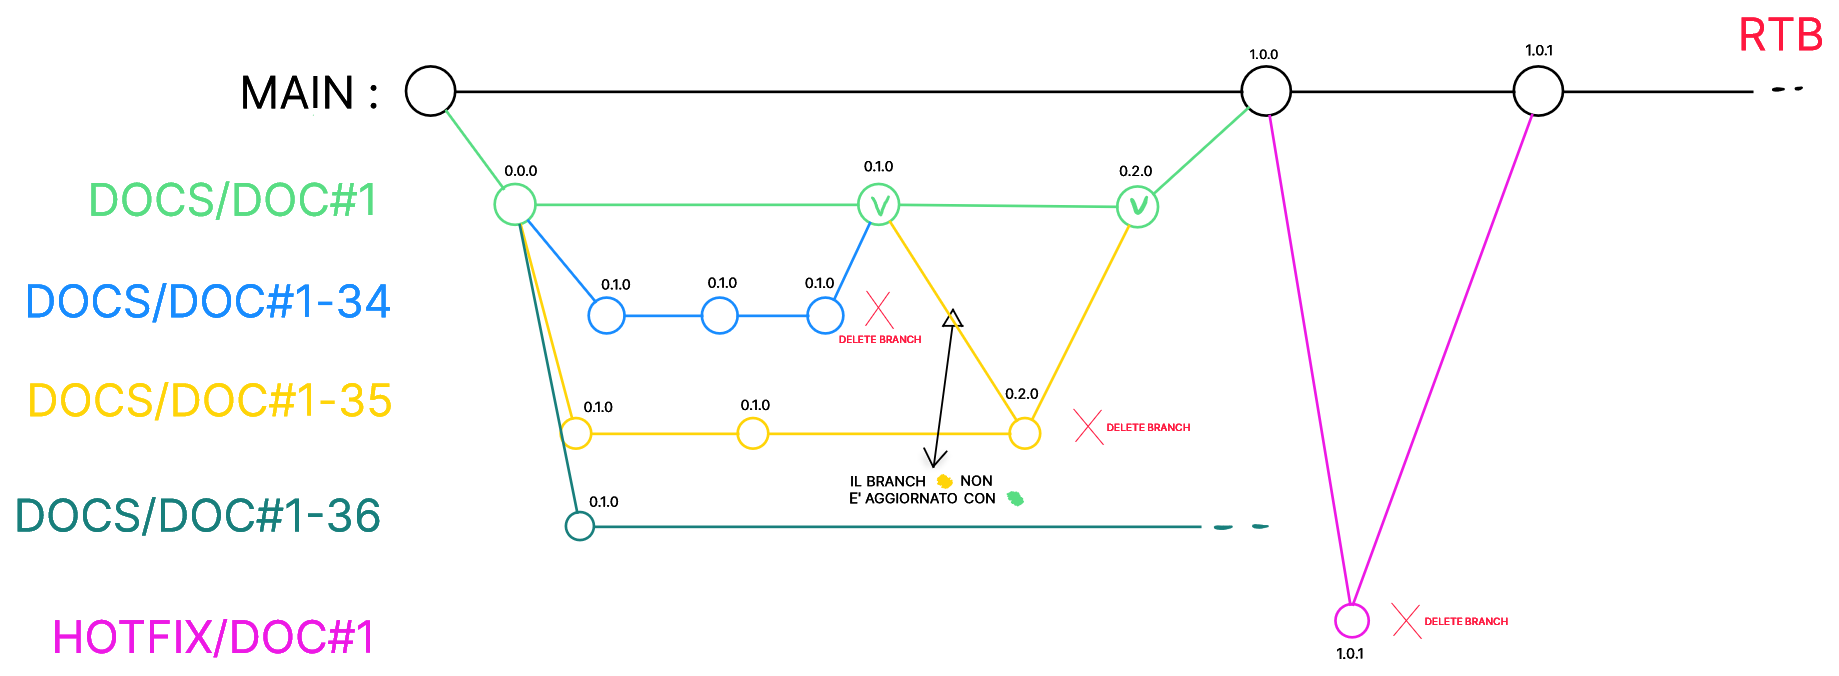
\includegraphics[scale = 0.33]{template/images/workflow.png}
\end{center}

\subsubsection{Commit}\label{inf:comm}
È preferibile che ogni commit abbia una singola responsabilità per cambiamento.
I commit non possono essere effettuati direttamente sui branch protetti ma per contribuire con delle aggiunte o
modifiche sarà necessario aprire una pull request, motivo per il quale abbiamo introdotto dei branch derivati.
I messaggi di commit dovranno seguire la seguenti strutture sintattiche:
\begin{center}
      \textbf{add: [COSA]\\
      change: [COSA]\\
      restructure: [COSA]}
\end{center}
dove:
\begin{itemize}
      \item \textbf{add}: viene utilizzato quando si va ad aggiungere una nuova sezione/sottosezione a un documento;
      \item \textbf{change}: viene utilizzato quando si va a modificare una o più sezioni/sottosezioni di un documento;
      \item \textbf{restructure}: indica una ristrutturazione del branch main per quanto riguarda l'organizzazione delle cartelle e/o la modifica di action o template di issue;
      \item \textbf{COSA}: breve descrizione di cosa di è aggiunto e/o fatto.
\end{itemize}

Dopo l'approvazione di una pull request tutti i commit relativi al documento
verranno raggruppati in un unico commit, il cui titolo deve rispettare la
struttura sintattica descritta in seguito.
\begin{center}
      \textbf{Update: [NOME-DOCUMENTO]-[VERSIONE]}
\end{center}
dove:

\begin{itemize}
      \item \textbf{NOME-DOCUMENTO}: indica il nome del documento nel quale sono state verificate le modifiche;
      \item \textbf{VERSIONE}: indica il numero di versione aggiornata.
\end{itemize}
Per quanto riguarda il commento facoltativo, si lascia quello di default proposto da GitHub,
ovvero un elenco puntato di tutti i commit che verranno raggruppati.\\

\subsubsection{Pull request}\label{inf:pr}
Per effettuare un merge su un branch protetto si deve aprire, da GitHub, una
pull request. Questa permette di verificare il lavoro svolto prima di
integrarlo con un branch protetto ed eseguire un veloce test di compilazione
della sezione aggiunta. Alla creazione di una pull request bisogna associare:
\begin{itemize}
      \item \textbf{Title}: [NOME-DOCUMENTO]-[ID-ISSUE];
      \item \textbf{Verificatori in carica}: coloro che hanno il compito di trovare eventuali errori o mancanze e fornire un feedback
            riguardante il contenuto direttamente su GitHub attraverso un commento, sulla stessa pull request.
            Non sarà possibile effettuare il merge finché tutti i commenti di revisione non saranno stati risolti
            con, al termine, l'approvazione di almeno uno dei verificatori e il test di build non dia esito positivo;
      \item \textbf{Descrizione}: contiene una lista riassuntiva di ciò che è stato fatto includendo le issue completate, e quindi da chiudere,
            con la sintassi
            \begin{center}
                  \textbf{close \#[ID-ISSUE]}
            \end{center}
            in modo tale che vengano tutte chiuse in automatico quando la pull request verrà accettata;
      \item \textbf{Gli assegnatari}: coloro che hanno anche il compito di apportare le modifiche necessarie al documento;
      \item \textbf{Label}: riassume di che natura è la pull request.
\end{itemize}
dove:

\begin{itemize}
      \item \textbf{NOME-DOCUMENTO}: indica il nome del documento sul quale si sta lavorando e richiedendo la verifica/approvazione;
      \item \textbf{ID-ISSUE}: indica il numero identificativo associato alla issue relativa alla modifica del documento.
\end{itemize}

Per una descrizione più dettagliata delle issue si faccia riferimento a
\nameref{inf:its}.

Per i commit relativi alle pull request seguire le regole descritte nella
sezione \nameref{inf:pr}.

\subsubsection{Automazioni}\label{inf:automaz}
\subsubsubsection{Scopo}
Lo scopo dell'automazione è garantire una maggiore efficienza e ridurre il
rischio di errori umani. Tuttavia, il costo necessario per rendere automatiche
alcune attività potrebbe essere superiore al beneficio ottenuto. È quindi
fondamentale scegliere attentamente quali processi automatizzare.
\subsubsubsection{Automazioni realizzate}
L'automazione dei processi di verifica e di compilazione della documentazione
avviene tramite GitHub Actions, che permette di eseguire script personalizzati
in risposta a eventi specifici che si verificano nel repository. In
particolare, sono state scritte tre diverse action:
\begin{itemize}
      \item \texttt{build.yml}: si scatena a seguito di un push sul main; ha il compito di compilare
            tutta la documentazione creata fino a quel momento e di creare la relativa pagina web tramite Pages;
      \item \texttt{pr\_build\_check.yml}: si scatena quando viene effettuata una pull request verso il main o verso
            un branch di documentazione, ovvero del tipo docs/[NOME-DOCUMENTO]. Serve per verificare che
            i sorgenti LaTeX compilino correttamente;
      \item \texttt{pr\_gulpease\_check.yml}: si scatena quando viene effettuata una pull request verso il main o verso
            un branch di documentazione, ovvero del tipo docs/[NOME-DOCUMENTO]. Essa verifica che
            l'indice Gulpease del documento, espresso come media degli indici delle sezioni, sia maggiore o uguale a 50.
\end{itemize}
Per garantire la qualità dei documenti prodotti, è necessario che le action \texttt{pr\_build\_check.yml}
e \\\texttt{pr\_gulpease\_check.yml} diano esito positivo. A tale scopo, è stato configurato il repository in modo
che non sia possibile effettuare il merge di una pull request se non sono soddisfatti entrambi i controlli.
Inoltre, per accelerare il processo di verifica, è fortemente raccomandato eseguire localmente gli script di test,
in modo da individuare e correggere eventuali errori prima di effettuare la pull request.
\subsubsubsection{Aggiungere un'action}
Per aggiungere un'action, è necessario seguire i seguenti passaggi:
\begin{itemize}
      \item Creare un file in linguaggio YAML nella cartella \texttt{.github/workflows} del
            repository, in cui si specificano i dettagli dell'action. In particolare, è
            necessario definirne:
            \begin{itemize}
                  \item Nome;
                  \item Evento che la scatena;
                  \item Job da eseguire;
                  \item Azioni da compiere all'interno di ciascun job.
            \end{itemize}
      \item Se necessario al funzionamento dell'automazione, produrre uno o più script e
            inserirli nella cartella \texttt{.github}. Il linguaggio utilizzato per
            scrivere tali script è python, scelto per la sua comprensibilità e facilità di
            utilizzo;
      \item Disabilitare temporaneamente il protection del main;
      \item Effettuare un commit con le modifiche apportate (vedi \nameref{inf:comm});
      \item Riabilitare il protection del main.
\end{itemize}

\subsubsection{Page Github}
\subsubsubsection{Scopo}
Attraverso la pagina GitHub, il team vuole fornire un punto di accesso centralizzato e di facile consultazione per tutta la documentazione.

\subsubsubsection{Aggiornare il sito}
Il procedimento è molto simile a quello per aggiungere un'action:
\begin{itemize}
      \item Modificare o creare un nuovo file in linguaggio HTML, CSS o Javascript nella cartella \texttt{website} del repository;
      \item Disabilitare temporaneamente il protection del main;
      \item Effettuare un commit con le modifiche apportate (vedi \nameref{inf:comm});
      \item Riabilitare il protection del main.
\end{itemize}

\subsubsection{Docker}
\subsubsubsection{Scopo}
Docker viene utilizzato per la creazione di immagini e container isolati per facilitare e velocizzare lo sviluppo dell'applicazione e garantendo portabilità e coerenza tra ambienti.

\subsubsubsection{Docker compose}
Sono stati creati 2 file per la creazione e avvio automatico dei container:
\begin{itemize}
      \item \textit{dc-dev.yaml:} permette la creazione di container che condividono volumi con l'host, consentendo l'hot-reloading immediato delle modifiche all'applicazione.
      \item \textit{dc-dep.yaml:}  permette la creazione di container che hanno una copia dell'applicazione, utilizzati per il deploy finale.
\end{itemize}


\subsection{Accertamento della qualità}
\subsubsection{Scopo}
Lo scopo del processo di accertamento della qualità è garantire la qualità dei
processi adottati e del software prodotto, al fine di soddisfare le aspettative
degli stakeholder e i requisiti del progetto. Ciò avviene tramite le attività
di pianificazione della qualità, il controllo della qualita e il miglioramento
continuo.
\subsubsection{Descrizione}
Il piano della qualità comprende gli obiettivi di qualità che il team si
impegna a raggiungere e le metriche utilizzate per misurare il raggiungimento
di tali obiettivi. \\ Il controllo della qualità consite nella misurazione e
analisi degli indicatori di interesse, valutando il grado di raggiungimento
degli obiettivi di qualità. \\ Il documento \textit{Piano di qualifica v1.1.0} tratta
nel dettaglio le attività di pianificazione e controllo della qualità. \\
\subsubsection{Ciclo di Deming}
Per quanto riguarda l'attività di miglioramento continuo dei processi, il
gruppo adotta il ciclo di Deming. Si tratta di un metodo di gestione iterativo
che prevede quattro fasi:
\begin{itemize}
      \item \textbf{Plan}: pianificazione degli obiettivi e dei processi necessari per fornire
            risultati in accordo con i risultati attesi, attraverso la creazione di attese di
            produzione, di completezza e accuratezza delle specifiche scelte;
      \item \textbf{Do}: attuazione del piano, tramite l'esecuzione dei processi,
            lo sviluppo dei prodotti e la misurazione dei risultati ottenuti;
      \item \textbf{Check}: analisi e studio dei dati raccolti nella fase Do.
            I grafici possono rendere più facile il confronto tra risultati ottenuti e attesi;
      \item \textbf{Act}: consolidamento delle soluzioni che hanno dato buoni risultati e
            adozione di strategie correttive per migliorare ciò che non ha soddisfatto le aspettative,
            dopo averne compreso a fondo le cause. In questo modo, ogni iterazione del ciclo di Deming
            contribuisce ad aggiungere valore al processo.
\end{itemize}
\subsubsection{Metriche}
Per perseguire la qualità nel processo di accertamento di qualità, si è deciso
di adottare le seguenti metriche:
\begin{itemize}
      \item \nameref{M:MM}.
\end{itemize}
\subsection{Verifica}
\subsubsection{Scopo}
Lo scopo del processo di verifica\textsubscript{g} è quello di accertare che
non siano stati commessi errori nello svolgimento delle attività prefissate.
Questo processo viene applicato costantemente sia durante la stesura della
documentazione, che durante lo sviluppo del software.
\subsubsection{Descrizione}
La verifica verrà fatta in maniera efficace adottando questi metodi:
\begin{itemize}
      \item \textbf{Analisi statica}: non richiede esecuzione dell'oggetto di verifica, quindi applicabile a documentazione e codice, usata per accertare conformità e regole nonché assenza di difetti, adotteremo i due seguenti metodi di lettura:
            \begin{itemize}
                  \item \textbf{Walkthrough}: il verificatore esamina documenti o codice in cerca di difetti, ma senza svolgere una
                        ricerca specifica per un certo tipo di errore. L'obiettivo è identificare errori, migliorare la qualità e favorire la comprensione;
                  \item \textbf{Inspection}: il verificatore controlla documenti o codice per trovare errori
                        eseguendo un'analisi mirata dell'oggetto di verifica. È necessario organizzare gli elementi da verificare in liste di controllo,
                        per poi passare alla verifica vera e propria. Questo approccio è più efficiente rispetto al walkthrough, 
                        anche perché in molti casi può essere automatizzato.
            \end{itemize}
      \item \textbf{Analisi dinamica}: richiede l'esecuzione dell'oggetto di verifica, quindi è applicabile solo al codice, usata per accertare che il codice sia corretto, non introduca errori nel sistema e soddisfi i requisiti preposti.
\end{itemize}
\subsubsection{Verifica della documentazione} Al momento della necessità di modificare o aggiungere qualcosa a una sezione di
un documento, si procederà in questo modo:
\begin{enumerate}
      \item Verrà creata una issue che specifica l'attività di modifica o aggiunta da
            svolgere;
      \item Verrà creato un sotto-branch\textsubscript{g} chiamato
            "docs/[NOME-DOCUMENTO]-N" dove con N si intende il numero della issue di
            riferimento;
      \item Rimanendo in questo sotto-branch\textsubscript{g}, verrà aggiornato il
            documento;
      \item Una volta terminato, per iniziare il processo di verifica\textsubscript{g}
            verrà aperta una pull request\textsubscript{g};
      \item Uno tra i verificatori in carica durante quello sprint si assegnerà la verifica
            del documento e modificherà il registro delle modifiche compilando il campo
            "Verificatore";
      \item Se la verifica avrà esito positivo, ci sarà il merge tra il
            sotto-branch\textsubscript{g} e il branch\textsubscript{g} principale del
            documento, con conseguente chiusura della issue e del sotto-branch;
      \item In caso di esito negativo, verranno segnalati gli errori da parte del
            verificatore tramite commenti, e il redattore si occuperà di risolverli
            continuando a lavorare nel sotto-branch\textsubscript{g}, fino ad avere il
            documento verificato.
\end{enumerate}

\subsubsection{Verifica del codice}
Il processo di verifica del codice si attua principalmente attraverso lo
sviluppo e l'esecuzione di test, che permettono di eseguire un'analisi dinamica
del software, ossia un'analisi che si concentra sul comportamento del programma
durante l'esecuzione. I test vengono progettati per garantire che il codice
funzioni correttamente in vari scenari e che rispetti i requisiti prefissati. I
principali tipi di test utilizzati in questo processo sono:
\begin{itemize}
      \item \textbf{Test di unità}: verificano il corretto funzionamento delle singole unità o funzioni del codice, testando piccoli blocchi di logica isolati.
            Questi test sono fondamentali per individuare errori precoci e garantire che ogni componente funzioni come previsto.
            Vengono definiti durante la progettazione di dettaglio;
      \item \textbf{Test di integrazione}: verificano che i vari moduli o componenti del sistema interagiscano correttamente tra loro.
            Questi test sono particolarmente utili per identificare problemi che si verificano quando le diverse parti del sistema vengono messe insieme.
            Vengono definiti nella fase di progettazione logica;
      \item \textbf{Test di regressione}: vengono eseguiti per verificare che le modifiche al codice non abbiano introducano nuovi errori o causino anomalie in funzionalità già presenti.
            Questi test sono essenziali per mantenere l'integrità del software durante lo sviluppo continuo;
      \item \textbf{Test di sistema}: testano il comportamento complessivo dell'applicazione in un ambiente che simula il più possibile l'ambiente di produzione.
            Questi test verificano che l'intero sistema funzioni come previsto sotto condizioni realistiche e che tutte le componenti siano correttamente integrate.
            Vengono definiti nella fase di analisi dei requisiti software;
\end{itemize}
I test vengono identificati attraverso un codice con questa struttura:
\textbf{
      \[
            T[\text{Tipo}][ \text{N}]
      \]
}
\\Dove N è il codice del test ed è un valore univoco e il tipo può essere:
\begin{itemize}
      \item \textbf{U}: test di unità;
      \item \textbf{I}: test di integrazione;
      \item \textbf{R}: test di regressione;
      \item \textbf{S}: test di sistema.
\end{itemize}
Ogni test, inoltre, possiede uno stato, che può essere:
\begin{itemize}
      \item \textbf{NI}: non implementato;
      \item \textbf{S}: superato;
      \item \textbf{NS}: non superato.
\end{itemize}
\paragraph{Metriche}
Per perseguire la qualità nel processo di verifica, si è deciso di adottare le
seguenti metriche:
\begin{itemize}
      \item \nameref{M:COC};
      \item \nameref{M:SC};
      \item \nameref{M:BC};
      \item \nameref{M:PTC};
      \item \nameref{M:LT};
      \item \nameref{M:ART};
      \item \nameref{M:CYC};
      \item \nameref{M:PPM};
      \item \nameref{M:LPM};
      \item \nameref{M:LPF};
      \item \nameref{M:CD}.
\end{itemize}
\subsection{Validazione}
Nel processo di validazione il fornitore dimostra che tutti i requisiti utente
sono stati soddisfatti. A tal fine assumono fondamentale importanza
i test di accettazione. Essi verificano che il prodotto finale sia conforme ai requisiti e
alle aspettative dell'utente finale, e quindi sia pronto per essere rilasciato.
I test di accettazione vengono definiti con il proponente nella fase di analisi dei requisiti.

\pagebreak

\section{Processi organizzativi}
Questa sezione mira a gestire i processi e il loro miglioramento,
l'organizzazione degli strumenti di supporto e la gestione del personale.

\subsection{Pianificazione}
\subsubsection{Metodo di Lavoro}
Il team ha adottato il metodo di lavoro Scrum, una delle metodologie Agile più
diffuse. Di conseguenza i compiti derivanti dai processi di sviluppo vengono
suddivisi in sprint di due settimane. Questo rende l'avanzamento del prodotto
più gestibile e più rapido, avendo però un tempo sufficiente per implementare
diverse feature e redigere i documenti necessari.
\paragraph*{Sprint}\label{inf:sprint} ~\\\\ Per ogni sprint, il responsabile
assegna i ruoli a ciascun membro, creando un diagramma delle attività per
stimare le ore necessarie e tenendo traccia dei giorni in cui ogni membro può
contribuire alla realizzazione del progetto. Successivamente, l'amministratore
si occuperà di creare le issue associate allo sprint in modo da rendere il
lavoro degli altri membri più semplice e veloce. Inoltre assicura che sia
avvenuta la verifica, in caso di modifica, del \textit{Piano di progetto} e
delle \textit{Norme di progetto} prima dell'inizio dello sprint successivo, in
modo da avere sempre la documentazione adatta e aggiornata sotto mano.\\\\ Le
attività dello sprint sono le seguenti:
\begin{itemize}
    \item \textbf{Sprint planning}:
          \begin{itemize}
              \item Il team definisce collettivamente le attività da svolgere durante lo sprint;
              \item Ogni componente del gruppo, durante la riunione, segnala le ore che può mettere
                    a disposizione;
              \item Il responsabile assegna i ruoli e definisce gli obiettivi dello sprint nel
                    documento \textit{Piano di progetto}.
          \end{itemize}
    \item \textbf{Daily scrum}: ogni giorno, i membri del team sono tenuti a condividere, attraverso il gruppo Telegram dedicato,
          un report dettagliato delle attività svolte il giorno precedente,
          quelle pianificate per la giornata in corso segnalando eventuali ostacoli che potrebbero compromettere il lavoro.
          Il responsabile controlla l'andamento dello sprint contattando i componenti del gruppo.
    \item \textbf{Sprint review}:
          \begin{itemize}
              \item Ogni membro, durante la riunione, riferisce quello che ha svolto nel periodo
                    precedente e gli eventuali dubbi che ha riscontrato;
              \item Viene fatta una lista degli obiettivi raggiunti e quelli non raggiunti.
          \end{itemize}
    \item \textbf{Sprint retrospective}: si fa una valutazione di quello che è andato bene durante lo sprint e di
          quello che è da migliorare, per capire come comportarsi per lo sprint successivo.
\end{itemize}

\subsubsection{Ruoli e responsabilità}
I membri del team \textit{Six Bit Busters} ricopriranno i ruoli principali di un
ciclo di vita del prodotto software, ovvero analista, progettista,
programmatore, verificatore, amministratore di sistema e responsabile. \\ Al
fine di garantire una comprensione completa delle diverse fasi e competenze
richieste nello sviluppo di un progetto, i membri del team ruoteranno
periodicamente tra i ruoli ogni due settimane. \\Questa rotazione periodica è
finalizzata a scopi didattici, permettendo a ciascun membro di acquisire una
visione globale del ciclo di vita del prodotto e di sviluppare abilità pratiche
in ogni area.
\begin{itemize}
    \item \textbf{Responsabile}\\
          Colui che coordina i membri del team e rappresenta il progetto verso l'esterno.
          Partecipa al progetto per tutta la sua durata.
          Le sue competenze sono:
          \begin{itemize}
              \item Preparare e presentare il \textit{Diario di bordo};
              \item Suddividere le attività del gruppo;
              \item Pianificare e gestire le risorse;
              \item Valutare rischi, scelte, alternative;
              \item Approvare i documenti prima di eseguire il merge nel branch main, aggiornando
                    la versione del documento e quindi andando ad incrementare il numero più a
                    sinistra.
          \end{itemize}
    \item \textbf{Amministratore di sistema}\\
          Colui che si occupa del funzionamento, mantenimento e sviluppo degli strumenti e ambienti tecnologici
          usati dal gruppo.
          Le sue competenze sono:
          \begin{itemize}
              \item Gestire le segnalazioni e problemi dei membri del gruppo relativi a
                    malfunzionamenti e difficoltà con gli strumenti tecnologici;
              \item Valutare l'utilizzo di nuove tecnologie e farne uno studio preliminare per
                    poter presentare al gruppo i pro e i contro del loro utilizzo;
              \item Controllare giornalmente la board e le issue per garantire una buona
                    organizzazione;
              \item Controllare se la documentazione è aggiornata;
              \item Presentare il \textit{Diario di bordo} in aula nel caso il responsabile non sia
                    presente;
              \item Redigere i verbali.
          \end{itemize}
          Ad ogni sprint si hanno al massimo due amministratori;
    \item \textbf{Analista}\\
          Colui che si occupa di analizzare a fondo il capitolato e le richieste del proponente per estrarne i requisiti.
          Le sue competenze sono:
          \begin{itemize}
              \item Studiare le richieste del proponente per identificare i requisiti e redigere
                    l'\textit{Analisi dei requisiti}.
          \end{itemize}
          Ad ogni sprint si ha almeno un analista;
    \item \textbf{Progettista}\\
          Colui che trasforma i requisiti, ricavati degli analisti, in una soluzione che abbia bassa complessità individuale.
          Le sue competenze sono:
          \begin{itemize}
              \item Prendere decisioni di natura tecnica e tecnologica riguardo lo sviluppo del
                    prodotto;
              \item Definire l'architettura del prodotto, in modo da soddisfare le specifiche;
              \item Sviluppare i diagrammi UML delle classi.
          \end{itemize}
    \item \textbf{Programmatore}\\
          Colui che si occupa di realizzare, tramite codice, il design presentato dal progettista.
          Le sue competenze sono:
          \begin{itemize}
              \item Scrivere il codice atto ad implementare i diagrammi delle classi;
              \item Scrivere eventuali test per il codice;
              \item Scrivere la documentazione per la comprensione del codice che scrive.
          \end{itemize}
    \item \textbf{Verificatore}\\
          Colui che si occupa di controllare che il lavoro degli altri membri del gruppo rispetti le \textit{Norme di progetto}
          prima che sia caricato in un branch protetto.
          Le sue competenze sono:
          \begin{itemize}
              \item Verificare che la documentazione e il codice scritto siano conformi alle
                    \textit{Norme di progetto};
              \item Proporre possibili migliorie da apportare a documenti e/o codice tramite dei
                    commenti.
          \end{itemize}
\end{itemize}

Per l'analisi dei ruoli e la rendicontazione delle ore preventivate si faccia
riferimento ai documenti \textit{Dichiarazione degli impegni} e \textit{Piano
    di progetto}.

\subsubsection{Metriche}
Per perseguire la qualità nel processo riguardo la pianificazione, si è deciso
di adottare le seguenti metriche:
\begin{itemize}
    \item \nameref{M:BV};
    \item \nameref{M:SV};
    \item \nameref{M:UR}.
\end{itemize}

\subsection{Modalità di comunicazione}
\subsubsection{Interne}
Si svolgono tra i soli componenti del gruppo. Si utilizza:
\begin{itemize}
    \item \textbf{Telegram}: canale di comunicazione asincrono per comunicazioni brevi;
    \item \textbf{Discord}: canale di comunicazione sincrono per le riunioni interne.
\end{itemize}
\subsubsection{Esterne}
Si svolgono tra il gruppo e una persona esterna, generalmente il proponente
o il committente. Si utilizza:
\begin{itemize}
    \item \textbf{Google Chat}: canale di comunicazione asincrono con il proponente;
    \item \textbf{Google Meet}: canale di comunicazione sincrono con il proponente;
    \item \textbf{GMail}: canale di comunicazione asincrono con il committente;
    \item \textbf{Zoom}: canale di comunicazione sincrono con il committente.
\end{itemize}

\subsection{Modalità di riunione}
\subsubsection{Interne}
Le riunioni interne si svolgono esclusivamente tra i membri del gruppo
utilizzando il canale apposito del server Discord. Per ogni riunione il
responsabile sarà incaricato di preparare una scaletta degli argomenti da
trattare, che potranno essere poi integrati da eventuali punti di discussione
portati dagli altri membri del gruppo.\\ Le riunioni si svolgono al termine di ogni sprint, cercando di trovare giorni e orari agevoli per tutti i membri del
gruppo. \\Al termine della riunione verrà redatto un verbale interno.

\subsubsection{Esterne}
Le riunioni esterne si svolgono tra i membri del gruppo e il proponente a
cadenza bisettimanale. Al termine della riunione verrà redatto un verbale
esterno.

\subsection{Gestione delle infrastrutture}
\subsubsection{Descrizione}
In questa sezione sono riportate le norme relative alla gestione delle
infrastrutture, vengono stabiliti gli strumenti di cui il gruppo farà uso e le
relative regole di utilizzo.

\subsubsection{GitHub}
Come servizio di hosting per il progetto il team ha optato per GitHub. \\Oltre
alla copia in remoto del repository del progetto, ogni membro del gruppo ha
una propria copia in locale nella quale può testare e fare prove senza
compromettere la struttura del progetto. \\Per prove più complesse è
consigliabile eseguire un fork del repository, in modo da avere una copia
identica del progetto anche in remoto sul proprio account personale.\\ 
Ogni membro può scaricare una copia del repository utilizzando Git ed
eseguendo uno dei seguenti comandi su Git bash o terminale Windows:
\begin{verbatim}
            git clone <git@github.com:6BitBusters/6BitBusters.github.io.git>
            git clone <https://github.com/6BitBusters/6BitBusters.github.io.git>
        \end{verbatim}
Il primo comando deve essere utilizzato se si impiegano le chiavi SSH per l'autenticazione, 
mentre il secondo è indicato per l'uso dei personal token.\\ Una volta completato il download verrà creata una cartella
collegata al repository del progetto in remoto.\\ Alternativamente, è possibile
eseguire le stesse operazioni tramite interfaccia grafica, con l'applicativo
GitHub Desktop.

\subsubsection{Overleaf}
Inizialmente, il team aveva scelto Overleaf come editor principale per la scrittura collaborativa di documenti online in LaTeX. 
Tuttavia, è emerso che non era la soluzione ottimale per la creazione dei documenti, soprattutto considerando l'automazione del processo di build implementata direttamente su GitHub. 
Attualmente Overleaf viene utilizzato esclusivamente come editor di supporto per i membri che non hanno installato LiveTeX in locale.

\subsubsection{Milestone}
Esistono 2 tipi di milestone:
\begin{itemize}
    \item \textbf{Interne}: indicano uno sprint;
    \item \textbf{Esterne}: indicano un traguardo intermedio significativo per il progetto.
\end{itemize}
Ad entrambe le milestone possono essere assegnate delle issue per verificarne il raggiungimento e per tenere traccia
della percentuale di progressione dello sprint.
Ogni milestone ha una scadenza che viene fissata da tutto il gruppo. Una delle prime milestone esterne create è
relativa alla Requirements and Technology Baseline e, di conseguenza, alla realizzazione di un PoC.

\subsubsection{Project board}\label{inf:pb}
È utilizzata un'unica project board per tracciare tutte le issue del repository, che funge da backlog del progetto. 
La project board è organizzata in quattro pannelli, che mostrano e raggruppano le issue in base alle loro caratteristiche.
\begin{itemize}
    \item \textbf{Board}: rappresenta le issue con un modello kanban;
    \item \textbf{Priority board}: simile alla Board ma ordina le issue in base alla loro priorità;
    \item \textbf{Team items}: rappresenta le issue tramite una lista verticale e rende possibile
          la modifica delle loro proprietà in modo semplice e veloce;
    \item \textbf{Roadmap}: rappresenta le issue in maniera simile a un diagramma di Gantt,
          dove in questo caso i task sono le singole issue.
\end{itemize}
Ad ogni issue è associato inoltre uno stato che viene utilizzato principalmente nei pannelli Board e Priority Board per una migliore gestione.
I possibili stati sono:
\begin{itemize}
    \item \textbf{Backlog}: issue che non sono ancora state iniziate o assegnate;
    \item \textbf{In progress}: issue che sono state assegnate e a cui almeno un membro, tra gli assegnatari, ha iniziato a lavorare;
    \item \textbf{Waiting for review}: issue terminate e che potrebbero essere chiuse definitivamente dopo la verifica delle modifiche apportate al documento;
    \item \textbf{In review}: issue terminate e in corso di verifica;
    \item \textbf{Done}: issue terminate e chiuse, con documenti o codice verificati.
\end{itemize}
Un esempio di workflow potrebbe essere il seguente:
\begin{enumerate}
    \item Viene creata la issue ed inserita all'interno della sezione ”Backlog” della
          Project board;
    \item Quando viene presa in carico, la issue viene spostata nella sezione ”In
          Progress” fino al suo completamento;
    \item L'incaricato, una volta risolta, apre una pull request a cui assegna la issue,
          come descritto nella sezione \nameref{inf:pr};
    \item Dopo l'approvazione della pull request la issue verrà chiusa e spostata in modo
          automatico nella sezione ”Done”.
\end{enumerate}

\subsubsection{Issue Tracking System}\label{inf:its}
Il gruppo utilizza l'issue tracking system di Github per tenere traccia delle
issue create. Le issue verranno create dall'amministratore, ma la loro
assegnazione verrà effettuata dai membri del gruppo in modo autonomo, in base
alla priorità, ruoli e disponibilità. Per marcare le issue secondo criteri di
interesse vengono utilizzate delle label:
\begin{itemize}
    \item \textbf{Correction}: indica una issue o pull request relativa ad una correzione alla documentazione;
    \item \textbf{Bug}: indica una issue o pull request relativa ad un errore/bug nel codice;
    \item \textbf{Code}: indica una issue o pull request relativa al codice;
    \item \textbf{Documentation}: indica una issue o pull request relativa alla documentazione;
    \item \textbf{Enhancement}: indica una issue o pull request relativa al miglioramento di scrittura documentazione o codice;
    \item \textbf{Wontfix}: indica una issue che verrà ignorata per motivi di tempo o perché punta ad una azione facoltativa.
\end{itemize}
Ogni issue, oltre alle label, possiede degli attributi aggiuntivi che permettono di arricchire
notevolmente la rappresentazione visiva sui pannelli, facilitando la comprensione e l'organizzazione del lavoro.
Si faccia riferimento alla sezione \nameref{inf:pb}.
Questi attributi sono:
\begin{itemize}
    \item \textbf{Estimate}: indica le ore stimate per completare il task descritto dalla issue;
    \item \textbf{Effective}: indica le ore effettive per completare il task descritto dalla issue;
    \item \textbf{Priority}: indica la priorità di una issue;
          \begin{itemize}
              \item \textbf{P0}: priorità alta;
              \item \textbf{P1}: priorità media;
              \item \textbf{P2}: priorità bassa.
          \end{itemize}
    \item \textbf{Begin}: indica la data entro la quale si deve iniziare a svolgere il task descritto dalla issue;
    \item \textbf{Due by}: indica la data entro la quale il task descritto dalla issue deve essere terminata.
\end{itemize}

Se un membro del gruppo si rende conto che la issue che sta
svolgendo potrebbe essere suddivisa in ulteriori issue, deve rivolgersi al
responsabile, il quale, se d'accordo, dà all'amministratore
il compito di modificare/aggiungere delle issue. Per rendere la
creazione delle issue più veloce e standardizzata, sono stati creati dei template in base al tipo di
issue che si vuole inserire e che richiedono degli input specifici.
\begin{itemize}
    \item  \textbf{TO-DO per documenti}
          \begin{itemize}
              \item \textbf{Titolo}: [NOME-DOCUMENTO]-[NOME-SEZIONE];
              \item \textbf{Oggetto di discussione} (facoltativo): [NOME-VERBALE];
              \item \textbf{Codice verbale}: il codice del tracciamento delle decisioni riportato a fine di ogni verbale;
              \item \textbf{Link verbale}: un collegamento ipertestuale al documento per accedervi direttamente;
              \item \textbf{Ruolo}: il ruolo che l'attività puntata dalla issue richiede;
              \item \textbf{Informazione da implementare}: lista di tutte le possibili parti della sezione da implementare.
          \end{itemize}
    \item  \textbf{To-DO per codice}
          \begin{itemize}
              \item \textbf{Titolo} : [CODICE-CASO-USO]-[NOME-FEATURE];
              \item \textbf{Oggetto di discussione} (facoltativo): [NOME-VERBALE];
              \item \textbf{Ruolo}: il ruolo che l'attività puntata dalla issue richiede;
              \item \textbf{Informazione da implementare}: breve descrizione di cosa, la feature aggiunta, deve fare o quali requisiti deve soddisfare.
          \end{itemize}
    \item  \textbf{Bug nel codice}
          \begin{itemize}
              \item \textbf{Titolo}: [CODICE-CASO-USO]-[NOME-FEATURE];
              \item \textbf{Descrizione bug}: breve descrizione del bug;
              \item \textbf{Passi per riprodurlo}: lista numerata per riassumere i passi da eseguire in modo tale che un'altro programmatore lo possa replicare;
              \item \textbf{Comportamento aspettato}: breve descrizione del comportamento aspettato;
              \item \textbf{Idea sul motivo} (facoltativo): se esiste, una veloce descrizione di un possibile motivo in modo tale da accelerare il processo di debug e correzione.
          \end{itemize}
    \item  \textbf{Correzione della documentazione}
          \begin{itemize}
              \item \textbf{Titolo} : [NOME-DOCUMENTO]-[NOME-SEZIONE];
              \item \textbf{Descrizione}: breve descrizione di cosa correggere nella sezione indicata.
          \end{itemize}
    \item  \textbf{Miglioramento della documentazione}
          \begin{itemize}
              \item \textbf{Titolo} : [NOME-DOCUMENTO]-[NOME-SEZIONE];
              \item \textbf{Descrizione}: breve descrizione di cosa modificare/migliorare e come, nella sezione indicata.
          \end{itemize}
    \item  \textbf{Miglioramento del codice}
          \begin{itemize}
              \item \textbf{Titolo} : [CODICE-CASO-USO]-[NOME-CASO-USO];
              \item \textbf{Descrizione}: breve descrizione di cosa modificare/migliorare e come, nella relativa parte di codice indicata.
          \end{itemize}
\end{itemize}
dove:

\begin{itemize}
    \item \textbf{NOME-DOCUMENTO}: indica il nome del documento sul quale si sta lavorando;
    \item \textbf{NOME-VERBALE}: indica il nome del verbale nel quale si è discusso della relativa attività rappresentata successivamente tramite una issue;
    \item \textbf{NOME-SEZIONE}: indica la sezione relativa al documento;
    \item \textbf{CODICE-CASO-USO}: indica il nome del caso d'uso nel quale si sta lavorando;
    \item \textbf{NOME-FEATURE}: indica il nome della feature relativa al caso d'uso.
\end{itemize}

\subsubsection{Discord}
Strumento utilizzato per la comunicazione, in modo sincrono, tra i componenti
del gruppo.\\ Sono stati creati diversi canali:
\begin{itemize}
    \item \textbf{Link} : canale testuale per avere dei collegamenti ipertestuali a risorse e riferimenti utili;
    \item \textbf{Utility} : canale testuale per la condivisione di media generici come loghi, disegni illustrativi per determinati workflow e appunti riguardanti le riunioni;
    \item \textbf{General}: canale vocale dedicato alle riunioni interne, al termine delle quali verrà redatto un verbale.
\end{itemize}

\subsubsection{Telegram}
Strumento utilizzato per la comunicazione, in modo asincrono, tra i componenti
del gruppo.\\ Sono stati creati 2 distinti gruppi:
\begin{itemize}
    \item \textbf{Generale} : gruppo dedicato alle comunicazioni brevi e poco importanti;
    \item \textbf{Daily scrum} : gruppo dedicato all'attivita di daily scrum, descritta nella sezione \nameref{inf:sprint}.
\end{itemize}

\subsection{Gestione dei dubbi e conflitti}
Nel caso sorgano dubbi, questi verranno risolti, in base all'urgenza, tramite
comunicazione nel canale Telegram o durante la riunione interna settimanale. \\
I conflitti invece verranno prevalentemente discussi in sede di riunione
interna, con l'obiettivo di trovare una soluzione condivisa che consenta al
progetto di progredire secondo una visione comune.


\pagebreak

\section{Standard per la qualità}

\subsection{ISO/IEC 12207:1995}
Per definire, misurare e valutare i processi da attuare nello svolgimento
del progetto, il gruppo adotta lo standard ISO/IEC 12207:1995, che
definisce un modello per i processi di ciclo di vita del software. 
Tale modello suddivide i processi in primari, di supporto e organizzativi.
Ogni processo consiste di più attività, e ogni attività è a sua volta
composta da più task.

\subsubsection{Processi primari}
I processi primari vengono impiegati dalle parti primarie durante il ciclo di 
vita del software. Una parte è detta primaria se avvia o si occupa dello 
sviluppo, dell'operatività o della manutenzione di prodotti software. 
Queste parti sono l'acquirente, il fornitore, lo sviluppatore, l'operatore e il manutentore.

\subsubsubsection{Acquisizione}
Processo che contiene le attività dell'acquirente, ossia l'organizzazione che
acquista un prodotto o servizio software.
\begin{itemize}
    \item Avviamento;
    \item Preparazione della richiesta di proposta;
    \item Preparazione e aggiornamento del contratto;
    \item Controllo dei fornitori;
    \item Accettazione e completamento.
\end{itemize}

\subsubsubsection{Fornitura}
Processo che contiene le attività del fornitore, ossia l'organizzazione che
fornisce il prodotto o servizio software all'acquirente.
\begin{itemize}
    \item Avviamento;
    \item Preparazione della risposta;
    \item Contratto;
    \item Pianificazione;
    \item Esecuzione e controllo;
    \item Revisione e valutazione;
    \item Consegna e completamento.
\end{itemize}

\subsubsubsection{Sviluppo}
Processo che contiene le attività dello sviluppatore, ossia l'organizzazione che
definisce, progetta e implementa il prodotto software.
\begin{itemize}
    \item Implementazione dei processi;
    \item Analisi dei requisiti di sistema;
    \item Progettazione dell'architettura di sistema;
    \item Analisi dei requisiti software;
    \item Progettazione dell'architettura software;
    \item Progettazione dettagliata del software;
    \item Codifica e test del software;
    \item Integrazione software;
    \item Integrazione di sistema;
    \item Installazione del software;
    \item Supporto all'accettazione del software.
\end{itemize}

\subsubsubsection{Processo operativo}
Processo che contiene le attività dell'operatore, ossia l'organizzazione che
fornisce il servizio di gestione del sistema informatico nel suo ambiente 
operativo per i suoi utenti.
\begin{itemize}
    \item Implementazione dei processi;
    \item Test operativo;
    \item Operazioni di sistema;
    \item Supporto utente.
\end{itemize}

\subsubsubsection{Manutenzione}
Processo che contiene le attività del manutentore, ossia l'organizzazione che
fornisce il servizio di manutenzione del prodotto software. Gestisce quindi 
le modifiche al prodotto software per mantenerlo aggiornato e in condizioni operative. 
\begin{itemize}
    \item Implementazione dei processi;
    \item Analisi dei problemi e delle modifiche;
    \item Implementazione delle modifiche;
    \item Revisione/accettazione delle manutenzione;
    \item Migrazione;
    \item Ritiro del software.
\end{itemize}

\subsubsection{Processi di supporto}
Un processo di supporto sostiene un altro processo come parte integrante 
con uno scopo distinto, e contribuisce al successo e alla qualità del progetto software. 
Un processo di supporto è impiegato ed eseguito, se necessario, da un altro processo. 

\subsubsubsection{Documentazione}
Processo per registrare le informazioni prodotte da un'attività o
da un processo di ciclo di vita.
\begin{itemize}
    \item Implementazione del processo;
    \item Progettazione e sviluppo;
    \item Produzione;
    \item Manutenzione.
\end{itemize}

\subsubsubsection{Gestione della configurazione}
Processo che consiste nell'applicare procedure amministrative e tecniche
attraverso il ciclo di vita del software allo scopo di identificare e definire
gli item in un sistema; controllare modifiche e rilasci degli item;
registrare lo stato degli item e le richieste di modifica; assicurare la completezza,
la consistenza e la correttezza degli item.
\begin{itemize}
    \item Implementazione del processo;
    \item Identificazione della configurazione;
    \item Controllo della configurazione;
    \item Resoconto dello stato della configurazione;
    \item Valutazione della configurazione;
    \item Gestione dei rilasci e delle consegne.
\end{itemize}

\subsubsubsection{Accertamento della qualità}
Processi per fornire adeguate garanzie che i processi e i prodotti
siano conformi ai requisiti e aderiscano ai piani stabiliti.
L'accertamento della qualità può utilizzare i risultati di altri
processi di supporto, come la verifica e la validazione.
\begin{itemize}
    \item Implementazione del processo;
    \item Accertamento dei prodotti;
    \item Accertamento dei processi;
    \item Accertamento dei sistemi di qualità.
\end{itemize}

\subsubsubsection{Verifica}
Processo per determinare se i prodotti di una data attività soddisfano
i requisiti e le condizione ad essi imposti nelle precedenti attività.
\begin{itemize}
    \item Implementazione del processo;
    \item Verifica.
\end{itemize}

\subsubsubsection{Validazione}
Processo per determinare se i requisiti e il sistema software
prodotto soddisfano la specifica destinazione d'uso.
\begin{itemize}
    \item Implementazione del processo;
    \item Validazione.
\end{itemize}

\subsubsubsection{Revisione congiunta}
Processo per valutare lo stato e i prodotti di un'attività, ove opportuno.
Le revisioni congiunte avvengono sia a livello di gestione di progetto che
a livello tecnico.
\begin{itemize}
    \item Implementazione del processo;
    \item Revisione della gestione di progetto;
    \item Revisione tecnica.
\end{itemize}

\subsubsubsection{Audit}
Processo per determinare la conformità con i requisiti, i piani 
e il contratto, ove opportuno.
\begin{itemize}
    \item Implementazione del processo;
    \item Audit.
\end{itemize}

\subsubsubsection{Risoluzione dei problemi}
Processo per analizzare e risolvere i problemi (incluse non conformità),
che si presentano durante l'esecuzione di altri processi. 
\begin{itemize}
    \item Implementazione del processo;
    \item Risoluzione dei problemi.
\end{itemize}

\subsubsection{Processi organizzativi}
I processi organizzativi vengono impiegati da un'organizzazione per stabilire 
e attuare una struttura di base costituita dai processi e dal personale,
e per migliorare costantemente tale struttura.

\subsubsubsection{Gestione organizzativa}
Processo che contiene le attività generiche che possono 
essere impiegate da qualunque parte che deve gestire i propri processi.
\begin{itemize}
    \item Avviamento e definizione dello scopo;
    \item Pianificazione;
    \item Esecuzione e controllo;
    \item Revisione e valutazione;
    \item Chiusura.
\end{itemize}

\subsubsubsection{Infrastruttura}
Processo per costruire e mantenere l'infrastruttura necessaria
agli altri processi.
\begin{itemize}
    \item Implementazione del processo;
    \item Costruzione dell'infrastruttura;
    \item Manutenzione dell'infrastruttura.
\end{itemize}

\subsubsubsection{Miglioramento}
Processo per definire, valutare, misurare, monitorare e migliorare
un processo di ciclo di vita.
\begin{itemize}
    \item Costituzione del processo;
    \item Valutazione del processo;
    \item Miglioramento del processo.
\end{itemize}

\subsubsubsection{Formazione}
Processo per fornire e mantenere personale adeguatamente formato.
\begin{itemize}
    \item Implementazione del processo;
    \item Sviluppo del materiale di formazione;
    \item Implementazione del piano di formazione.
\end{itemize}

\subsection{ISO/IEC 9126}
Per definire, misurare e valutare il software prodotto, il gruppo adotta lo 
standard ISO/IEC 9126, che definisce un modello di qualità del software. Tale 
modello è organizzato in sei caratteristiche principali, 
ognuna delle quali è suddivisa in sottocaratteristiche.

\subsubsection{Funzionalità}
La funzionalità misura la capacità del software di soddisfare i requisiti specificati e di fornire le funzioni,
espresse e implicite, necessarie per operare in un determinato contesto.
\begin{itemize}
    \item \textbf{Appropriatezza}: capacità di eseguire i compiti richiesti;
    \item \textbf{Accuratezza}: livello di correttezza dei risultati;
    \item \textbf{Interoperabilità}: capacità di interagire con uno o più sistemi specificati;
    \item \textbf{Sicurezza}: protezione delle informazioni e dei dati da accessi non autorizzati;
    \item \textbf{Conformità}: adesione a standard, convenzioni e regolamenti relativi alla funzionalità.
\end{itemize}

\subsubsection{Affidabilità}
L'affidabilità misura la capacità del software di svolgere correttamente il suo compito
mantenendo un certo livello di prestazioni quando usato in determinate condizioni.
\begin{itemize}
    \item \textbf{Maturità}: capacità di evitare errori, malfunzionamenti e guasti;
    \item \textbf{Tolleranza agli errori}: capacità di mantenere un certo livello di prestazioni anche in presenza di errori;
    \item \textbf{Recuperabilità}: capacità di ripristinare il livello di prestazioni e di recuperare
        i dati in caso di errori;
    \item \textbf{Conformità}: adesione a standard, convenzioni e regolamenti relativi all'affidabilità.
\end{itemize}

\subsubsection{Efficienza}
L'efficienza misura la capacità del software di offrire prestazioni adeguate in relazione alle risorse impiegate.
Le risorse includono altri prodotti software e la configurazione hardware e software del sistema.
\begin{itemize}
    \item \textbf{Comportamento rispetto al tempo}: velocità di risposta ed elaborazione;
    \item \textbf{Utilizzo delle risorse}: capacità di utilizzare un appropriato numero e tipo di risorse;
    \item \textbf{Conformità}: adesione a standard, convenzioni e regolamenti relativi all'efficienza.
\end{itemize}

\subsubsection{Usabilità}
L'usabilità misura la capacità del software di essere comprensibile, di poter essere
studiato e di risultare attraente per un utente sotto determinate condizioni.
\begin{itemize}
    \item \textbf{Comprensibilità}: capacità di essere compreso facilmente;
    \item \textbf{Apprendibilità}: facilità di apprendimento delle funzionalità;
    \item \textbf{Operabilità}: facilità di essere utilizzato e controllato;
    \item \textbf{Attrattività}: capacità di essere attraente per l'utente;
    \item \textbf{Conformità}: adesione a standard, convenzioni e regolamenti relativi all'usabilità.
\end{itemize}

\subsubsection{Manutenibilità}
La manutenibilità misura la capacità del software di essere adattato per 
correggere errori, implementare miglioramenti o rispondere a cambiamenti 
negli ambienti e nei requisiti.

\begin{itemize}
    \item \textbf{Analizzabilità}: facilità di diagnosticare problemi;
    \item \textbf{Modificabilità}: capacità di essere modificato;
    \item \textbf{Stabilità}: capacità di mantenere il funzionamento dopo modifiche;
    \item \textbf{Testabilità}: facilità di eseguire test sul software;
    \item \textbf{Conformità}: adesione a standard, convenzioni e regolamenti relativi alla manutenibilità.
\end{itemize}

\subsubsection{Portabilità}
La portabilità misura la capacità del software di essere trasferito da un ambiente di lavoro a un altro.
L'ambiente include aspetti organizzativi e tecnologici (hardware e software).
\begin{itemize}
    \item \textbf{Adattabilità}: capacità di adattarsi a diversi ambienti di lavoro;
    \item \textbf{Installabilità}: facilità di installazione;
    \item \textbf{Coesistenza}: capacità di coesistere con altri software;
    \item \textbf{Sostituibilità}: facilità con cui il software può sostituirne un altro, per lo 
        stesso scopo e nello stesso ambiente;
    \item \textbf{Conformità}: adesione a standard, convenzioni e regolamenti relativi alla portabilità.
\end{itemize}
\pagebreak

\newcounter{M}

\newcommand{\MPC}[2]{
    \refstepcounter{M}
    \subsubsection{MPC\arabic{M} - #1}\label{M:#2}
    }
\newcommand{\MPD}[2]{
    \refstepcounter{M}
    \subsubsection{MPD\arabic{M} - #1}\label{M:#2}
}
\GetTitleStringSetup{expand}
\section{Metriche di qualità}
\subsection{Introduzione}
Le metriche di qualità sono strumenti fondamentali per
valutare e migliorare l’efficacia e l’efficienza nello sviluppo del software. Queste metriche
forniscono indicatori oggettivi e misurabili che consentono di valutare la conformità agli
standard, identificare aree di miglioramento e monitorare la salute complessiva del processo
di sviluppo.
\subsection*{Codifica}
\begin{center}
    \textbf{M[Tipologia][Id numerico]}
\end{center}
dove:
\begin{itemize}
    \item \textbf{Tipologia}: indica il tipo della metrica:
    \begin{itemize}
        \item \textbf{PC}: per il processo;
        \item \textbf{PD}: per il prodotto.
    \end{itemize}
    \item \textbf{Id numerico}: indica un numero univoco incrementale separato per le due tipologie.
\end{itemize}


\subsection{Metriche per la qualità di processo}
Di seguito sono descritte le metriche di qualità di processo che il gruppo intende adottare.
\MPC{Planned Value (PV)}{PV}
Costo pianificato (in \euro) per realizzare le attività di progetto alla data corrente.
\begin{itemize}
    \item \textbf{Formula}: $PV = BAC * \frac{PH}{THP}$
    \item \textbf{Valore accettabile}: $\geq0$ \euro
    \item \textbf{Valore ottimale}: $\leq$ BAC
\end{itemize}  
Per eseguire il calcolo:
\begin{itemize}
    \item \textbf{BAC}: il budget totale preventivato;
    \item \textbf{PH}: ore di lavoro pianificate;
    \item \textbf{THP}: ore di lavoro pianificate totali.
\end{itemize}

\MPC{Actual Cost (AC)}{AC}
Costo effettivamente sostenuto (in \euro) alla data corrente. 
\begin{itemize}
    \item \textbf{Formula}: $AC = \sum_{r}^{R}(THR_r*HC_r)$
    \item \textbf{Valore accettabile}: $\geq0$ \euro
    \item \textbf{Valore ottimale}: $\leq$ EaC (Estimated at Completion)
\end{itemize}  
Per eseguire il calcolo:
\begin{itemize}
    \item \textbf{R}: insieme dei ruoli;
    \item \textbf{THR}: ore di lavoro effettive per ruolo;
    \item \textbf{HC}: costo fisso ad ora per il determinato ruolo.
\end{itemize}

\MPC{Earned Value (EV)}{EV}
Valore (in \euro) delle attività realizzate nel progetto fino alla data corrente. 
\begin{itemize}
    \item \textbf{Formula}: $EV=BAC*\frac{EH}{THP}$
    \item \textbf{Valore accettabile}: $\geq0$ \euro
    \item \textbf{Valore ottimale}: $\leq$ EaC
\end{itemize}  
Per eseguire il calcolo:
\begin{itemize}
    \item \textbf{BAC} : il budget totale preventivato;
    \item \textbf{EH}: ore di lavoro effettive;
    \item \textbf{THP}: ore di lavoro pianificate totali.
\end{itemize}

\MPC{Estimated at Completion (EaC)}{EAC}
Revisione del costo (in \euro) stimato per la realizzazione del progetto alla data corrente. 
\begin{itemize}
    \item \textbf{Formula}:$EaC = AC+EtC$
    \item \textbf{Valore accettabile}: $\geq BAC - 5\%$
    \item \textbf{Valore accettabile}: $\leq  BAC + 5\%$
    \item \textbf{Valore ottimale}: BAC
\end{itemize}  
Per eseguire il calcolo:
\begin{itemize}
    \item \textbf{AC}: Actual Cost;
    \item \textbf{EtC}: Estimated to Complete.
\end{itemize}


\MPC{Estimate to Complete (EtC)}{ETC}
Valore (in \euro) stimato per la realizzazione delle rimanenti attività necessarie al completamento del progetto. 
\begin{itemize}
    \item \textbf{Formula}: $EtC=BAC-EV$
    \item \textbf{Valore accettabile}: $\geq0$ \euro
    \item \textbf{Valore ottimale}: $\leq$ EaC
\end{itemize}  
Per eseguire il calcolo:
\begin{itemize}
    \item \textbf{BAC}: il budget totale preventivato;
    \item \textbf{EV}: Earned Value.
\end{itemize}

\MPC{Cost Variance (CV)}{CV}
Valore che indica se del costo realmente maturato è maggiore, uguale o minore rispetto al costo effettivo.
Se CV $>$ 0 , il progetto è più efficiente (costo inferiore rispetto a quanto pianificato); 
se CV $<$ 0 , il progetto è meno efficiente (costo superiore rispetto a quanto pianificato). 
Se CV = 0 , il progetto rispetta esattamente il costo pianificato.
\begin{itemize}
    \item \textbf{Formula}: $CV=EV-AC$
    \item \textbf{Valore accettabile}: $\geq0$ \euro
    \item \textbf{Valore ottimale}: $\geq0$ \euro
\end{itemize}  
Per eseguire il calcolo:
\begin{itemize}
    \item \textbf{AC} : Actual Cost;
    \item \textbf{EV}: Earned Value.
\end{itemize}

\MPC{Schedule Variance (SV)}{SV}
Percentuale che indica se si è in linea, in anticipo o in ritardo rispetto alla schedulazione delle attività di progetto pianificate nella baseline. 
Se SV $>$ 0 significa che il progetto sta producendo con maggior velocità a quanto pianificato, viceversa se negativo. 
\begin{itemize}
    \item \textbf{Formula}: $SV=\frac{EV-PV}{PV}*100$
    \item \textbf{Valore accettabile}: $\geq-10\%$
    \item \textbf{Valore ottimale}: $\geq0\%$
\end{itemize}  
Per eseguire il calcolo:
\begin{itemize}
    \item \textbf{EV}: Earned Value;
    \item \textbf{PV}: Planned Value.
\end{itemize}

\MPC{Budget Variance (BV)}{BV}
Percentuale che indica se alla data corrente si è speso di più o di meno rispetto a quanto previsto a budget alla data corrente. 
Se BV $>$ 0 significa che il progetto sta spendendo il proprio budget con maggior velocità di quanto pianificato, viceversa se negativo.
\begin{itemize}
    \item \textbf{Formula}: $BV=\frac{PV-AC}{PV}*100$
    \item \textbf{Valore accettabile}: $-10\%\leq BV \leq 10\%$
    \item \textbf{Valore ottimale}: $0\%$
\end{itemize}  
Per eseguire il calcolo:
\begin{itemize}
    \item \textbf{AC} : Actual Cost;
    \item \textbf{PV}: Planned Value.
\end{itemize}

\MPC{Requirements Stability Index (RSI)}{RSI}
Indice che traccia la variazione dei requisiti dell'arco del progetto
\begin{itemize}
    \item \textbf{Formula}: $RSI = (1 - \frac{CRN+DRN+ARN}{IR})*100$
    \item \textbf{Valore accettabile}: $\geq70\%$
    \item \textbf{Valore ottimale}: $100\%$
\end{itemize}  
Per eseguire il calcolo:
\begin{itemize}
    \item \textbf{CRN} : numero di requisiti cambiati;
    \item \textbf{DRN}: numero di requisiti eliminati;
    \item \textbf{ARN}: numero di requisiti aggiunti;
    \item \textbf{IR}: numero totale di requisiti iniziali.
\end{itemize}

\MPC{Completezza dei documenti}{DOCC}
Percentuale che indica lo stato di completezza di un documento
\begin{itemize}
    \item \textbf{Formula}: $CD=\frac{SS}{TS}*100$
    \item \textbf{Valore accettabile}: $100\%$
    \item \textbf{Valore ottimale}: $100\%$
\end{itemize} 
Per eseguire il calcolo:
\begin{itemize}
    \item \textbf{SS}: sezioni del documento redatte;
    \item \textbf{TS}: sezioni del documento da redigere;
\end{itemize} 


\MPC{Metriche soddisfatte}{MM}
Indice percentuale per tenere conto delle metriche soddisfatte. Una
metrica si dice soddisfatta se raggiunge almeno il valore accettabile imposto sul \textit{Piano di Qualifica}.
\begin{itemize}
    \item \textbf{Formula}: $MS = \frac{MS}{TM}*100$
    \item \textbf{Valore accettabile}:$\geq80\%$
    \item \textbf{Valore ottimale}:$100\%$
\end{itemize}  
Per eseguire il calcolo:
\begin{itemize}
    \item \textbf{MS} : numero di metriche soddisfatte;
    \item \textbf{TM}: numero di metriche valutate.
\end{itemize}

\MPC{Code Coverage}{COC}
Percentuale che indica quanta porzione di codice sorgente è stata eseguita tramite test.
\begin{itemize}
    \item \textbf{Valore accettabile}:$\geq75\%$
    \item \textbf{Valore ottimale}:$\geq90\%$
\end{itemize} 

\MPC{Statement Coverage (SC)}{SC} 
Percentuale che indica quante istruzioni del codice che sono state eseguite tramite test.
\begin{itemize}
    \item \textbf{Formula}: $SC = \frac{ES}{TS}*100$
    \item \textbf{Valore accettabile}: $\geq80\%$
    \item \textbf{Valore ottimale}: $100\%$
\end{itemize}  
Per eseguire il calcolo:
\begin{itemize}
    \item \textbf{ES} : numero di linee eseguite;
    \item \textbf{TS}: numero di linee totali;
\end{itemize}

\MPC{Branch Coverage (BC)}{BC} 
Percentuale che indica i rami di decisione nel codice che sono stati eseguiti tramite test.
\begin{itemize}
    \item \textbf{Formula}: $BC = \frac{EB}{TB}*100$
    \item \textbf{Valore accettabile}: $\geq80\%$
    \item \textbf{Valore ottimale}: $100\%$
\end{itemize}  
Per eseguire il calcolo:
\begin{itemize}
    \item \textbf{EB} : numero di rami eseguiti;
    \item \textbf{TB}: numero di rami totali;
\end{itemize}

\MPC{Rischi non previsti}{UR}
Valore intero che indica il numero di rischi non previsti durante il corso del progetto.
\begin{itemize}
    \item \textbf{Valore accettabile}: $\leq5$
    \item \textbf{Valore ottimale}: $0$
\end{itemize}  


\pagebreak
\setcounter{M}{0}
\subsection{Metriche per la qualità di prodotto}
Di seguito sono descritte le metriche di qualità di prodotto che il gruppo intende adottare.

\MPD{Indice Gulpease}{GI}
Indice di leggibilità di un testo tarato sulla lingua italiana. I risultati sono compresi tra 0 e
100, dove il valore 100 indica la leggibilità più alta e 0 la leggibilità più bassa. Ai seguenti valori si
associano i seguenti significati:
\begin{itemize}
    \item inferiore a 80 sono difficili da leggere per chi ha la licenza elementare;
    \item inferiore a 60 sono difficili da leggere per chi ha la licenza media;
    \item inferiore a 40 sono difficili da leggere per chi ha un diploma superiore.
\end{itemize}
\begin{itemize}
    \item \textbf{Formula}: $GI=89+\frac{300*PN-10*LN}{WN}$
    \item \textbf{Valore accettabile} $\geq50$
    \item \textbf{Valore ottimale}: $\geq80$
\end{itemize}  
Per eseguire il calcolo:
\begin{itemize}
    \item \textbf{PN} : numero di frasi;
    \item \textbf{LN}: numero di lettere;
    \item \textbf{WN}: numero di parole.
\end{itemize}

\MPD{Errori grammaticali}{GE}
Numero di errori grammaticali presenti nei documenti.
\begin{itemize}
    \item \textbf{Valore accettabile} $0$
    \item \textbf{Valore ottimale}: $0$
\end{itemize}  

\MPD{Requisiti obbligatori soddisfatti}{MR}
Percentuale che indica i requisiti obbligatori soddisfatti.
\begin{itemize}
    \item \textbf{Formula}: $CMR=\frac{MR}{TMR}*100$
    \item \textbf{Valore accettabile}: 100\%
    \item \textbf{Valore ottimale}: 100\%
\end{itemize}
Per eseguire il calcolo:
\begin{itemize}
    \item \textbf{MR} : numero di requisiti obbligatori soddisfatti;
    \item \textbf{TMR}: numero di requisiti obbligatori in totale.
\end{itemize} 

\MPD{Requisiti desiderabili soddisfatti}{DR}
Percentuale che indica i requisiti desiderabili soddisfatti.
\begin{itemize}
    \item \textbf{Formula}: $CDR=\frac{DR}{TDR}*100$
    \item \textbf{Valore accettabile}: $\geq0\%$
    \item \textbf{Valore ottimale}: $100\%$
\end{itemize}  
Per eseguire il calcolo:
\begin{itemize}
    \item \textbf{DR} : numero di requisiti desiderabili soddisfatti;
    \item \textbf{TDR}: numero di requisiti desiderabili in totale.
\end{itemize} 


\MPD{Requisiti opzionali soddisfatti}{OR}
Percentuale che indica i requisiti opzionali soddisfatti.
\begin{itemize}
    \item \textbf{Formula}: $COR=\frac{OR}{TOR}*100$
    \item \textbf{Valore accettabile}: $\geq0\%$
    \item \textbf{Valore ottimale}: $100\%$
\end{itemize}  
Per eseguire il calcolo:
\begin{itemize}
    \item \textbf{OR} : numero di requisiti opzionali soddisfatti;
    \item \textbf{TOR}: numero di requisiti opzionali in totale.
\end{itemize} 

\MPD{Casi di test superati}{PTC}
Percentuale che indica i test che terminano con esisto positivo.
\begin{itemize}
    \item \textbf{Formula}: $CTS=\frac{PTC}{TTC}*100$
    \item \textbf{Valore accettabile}: $\geq90\%$
    \item \textbf{Valore ottimale}: $100\%$
\end{itemize}
Per eseguire il calcolo:
\begin{itemize}
    \item \textbf{PTC} : numero di test superati;
    \item \textbf{TTC}: numero di test in totale.
\end{itemize} 

\MPD{Densità errori}{FD}
Percentuale di failure o di esecuzioni non andate a buon fine di determinate azioni. Le
eventuali esecuzioni fallite o failure saranno segnate dai programmatori e di conseguenza verrà calcolato
il valore della metrica.
\begin{itemize}
    \item \textbf{Formula}: $FD=\frac{FTN}{TN}*100$
    \item \textbf{Valore accettabile}: 20\%
    \item \textbf{Valore ottimale}: 10\%
\end{itemize}  
Per eseguire il calcolo:
\begin{itemize}
    \item \textbf{FTN} : numero di test falliti;
    \item \textbf{TN}: numero di test eseguiti in totale.
\end{itemize}

\MPD{Tempo di apprendimento}{EOL}
Misura basata sul tempo che rappresenta quando, in media, un'utente ci impiega per imparare come si utilizza il programma.
\begin{itemize}
    \item \textbf{Valore accettabile}: $\leq$ 5 minuti;
    \item \textbf{Valore ottimale}: $\leq$ 2 minuti;
\end{itemize}  

\MPD{Tempo di caricamento}{LT}
Tempo medio di attesa per il caricamento dell'applicazione.
\begin{itemize}
    \item \textbf{Valore accettabile}:$\leq15$ secondi
    \item \textbf{Valore ottimale}:$\leq10$ secondi
\end{itemize} 

\MPD{Tempo medio di risposta}{ART}
Tempo medio impiegato dal software per rispondere a una richiesta utente o svolgere un’attività di sistema. 
\begin{itemize}
    \item \textbf{Valore accettabile}:$\leq5$ secondi
    \item \textbf{Valore ottimale}:$\leq1$ secondi
\end{itemize}  

\MPD{Complessità ciclomatica}{CYC}
Metrica utilizzata per misurare la complessità di un singolo metodo. Calcolata sul grafo dei cammini linearmente indipendenti percorsi dal software ed i punti decisionali del programma.
\begin{itemize}
    \item \textbf{Formula}: $CC=v(G)=e-n+2p$
    \item \textbf{Valore accettabile}: $\leq8$
    \item \textbf{Valore ottimale}: $\leq4$
\end{itemize}  
Per eseguire il calcolo:
\begin{itemize}
    \item \textbf{e} : numero di archi nel grafo;
    \item \textbf{n}: numero di punti decisionali (nodi) nel grafo;
    \item \textbf{p}: numero di componenti connesse tra loro.
    \item \textbf{G}: grafo dei cammini.
\end{itemize}

\MPD{Parametri per metodo}{PPM}
Valore che indica quanti parametri può avere un metodo all'interno del codice sorgente.
\begin{itemize}
    \item \textbf{Valore accettabile}: $\leq6$
    \item \textbf{Valore ottimale}: $\leq4$
\end{itemize} 

\MPD{Linee di codice per metodo}{LPM}
Valore che indica da quante linee di codice può essere composto un metodo all'interno del codice sorgente.
\begin{itemize}
    \item \textbf{Valore accettabile}: $\leq30$
    \item \textbf{Valore ottimale}: $\leq20$
\end{itemize} 

\MPD{Linee di codice per file}{LPF}
Valore che indica da quante linee di codice può essere composto un file nel progetto.
\begin{itemize}
    \item \textbf{Valore accettabile}: $\leq120$
    \item \textbf{Valore ottimale}: $\leq80$
\end{itemize} 

\MPD{Densità dei commenti}{CD}
Percentuale delle righe di commento sul totale delle righe di codice presenti in un modulo.
\begin{itemize}
    \item \textbf{Formula}: $CD=\frac{CMLN}{CLN}*100$
    \item \textbf{Valore accettabile}: $20-45\%$
    \item \textbf{Valore ottimale}: $25-35\%$
\end{itemize}  
Per eseguire il calcolo:
\begin{itemize}
    \item \textbf{CMLN}: numero di righe di commento;
    \item \textbf{CLN}: numero di righe di codice.
\end{itemize}

\MPD{Supported Browser(SB)}{SB}
Valore percentuale dei browser e loro relativa versione che supportano dal prodotto software.
\begin{itemize}
    \item \textbf{Formula}: $SB=\frac{BN}{TBN}*100$
    \item \textbf{Valore accettabile}: $\geq80\%$
    \item \textbf{Valore ottimale}: $100\%$
\end{itemize}  
Per eseguire il calcolo:
\begin{itemize}
    \item \textbf{BN} : numero di browser in cui il software funziona;
    \item \textbf{TBN}: numero di browser testati.
\end{itemize}


\pagebreak

\end{document}


